%% bare_conf.tex
%% V1.2
%% 2002/11/18
%% by Michael Shell
%% mshell@ece.gatech.edu
%%
%% NOTE: This text file uses MS Windows line feed conventions. When (human)
%% reading this file on other platforms, you may have to use a text
%% editor that can handle lines terminated by the MS Windows line feed
%% characters (0x0D 0x0A).
%%
%% This is a skeleton file demonstrating the use of IEEEtran.cls
%% (requires IEEEtran.cls version 1.6b or later) with an IEEE conference paper.
%%
%% Support sites:
%% http://www.ieee.org
%% and/or
%% http://www.ctan.org/tex-archive/macros/latex/contrib/supported/IEEEtran/
%%
%% This code is offered as-is - no warranty - user assumes all risk.
%% Free to use, distribute and modify.
% *** Authors should verify (and, if needed, correct) their LaTeX system  ***
% *** with the testflow diagnostic prior to trusting their LaTeX platform ***
% *** with production work. IEEE's font choices can trigger bugs that do  ***
% *** not appear when using other class files.                            ***
% Testflow can be obtained at:
% http://www.ctan.org/tex-archive/macros/latex/contrib/supported/IEEEtran/testflow

% Note that the a4paper option is mainly intended so that authors in
% countries using A4 can easily print to A4 and see how their papers will
% look in print. Authors are encouraged to use U.S. letter paper when
% submitting to IEEE. Use the testflow package mentioned above to verify
% correct handling of both paper sizes by the author's LaTeX system.
%
% Also note that the "draftcls" or "draftclsnofoot", not "draft", option
% should be used if it is desired that the figures are to be displayed in
% draft mode.
%
% This paper can be formatted using the peerreviewca
% (instead of conference) mode.
%\documentclass[conference]{IEEEtran}
%\documentclass[10pt,conference,compsocconf,letterpaper]{IEEEtran}
\documentclass[10pt, conference, letterpaper]{IEEEtran}
%\usepackage{CTEX}
%\usepackage{algorithm}
%\usepackage[noend]{algorithmic}
\usepackage{algorithmic}
\usepackage[ruled,vlined,linesnumbered]{algorithm2e}
\usepackage{url}
\usepackage{verbatim} % multi-line comments
\usepackage{multirow}
\usepackage{upgreek}
\usepackage{amsthm}
\newtheorem{example}{\noindent{\bf Example}}
\newtheorem{definition}{\noindent{\bf Definition}}
\newtheorem{lemma}{\noindent{\bf Lemma}}
\newtheorem{theorem}{\noindent{\bf Theorem}}
\newtheorem{corollary}{\noindent{\bf Corollary}}
\newtheorem{conjecture}{\noindent{\bf Conjecture}}
\newcommand{\tabincell}[2]{\begin{tabular}{@{}#1@{}}#2\end{tabular}}
\newcommand{\tickYes}{\checkmark}
\newcommand{\tickNo}{\hspace{1pt}\ding{56}}
\newcommand{\bm}[1]{\mbox{\boldmath{$#1$}}} % boldmath

\renewcommand{\labelitemi}{$\bullet$}
% algorithm
\renewcommand{\algorithmicrequire}{\textbf{Input:}}
\renewcommand{\algorithmicensure}{\textbf{Output:}}
\renewcommand{\algorithmiccomment}[1]{// #1}
\newcommand{\INDSTATE}[1][1]{\STATE\hspace{#1\algorithmicindent}}
%\newcommand\AND{\textbf{and} }

\usepackage{pifont} % for tickNo
%\usepackage[caption=false,font=footnotesize]{subfig} % subfig
%\usepackage{graphicx}
%\usepackage{subfigure}
% If the IEEEtran.cls has not been installed into the LaTeX system files,
% manually specify the path to it:
% \documentclass[conference]{../sty/IEEEtran}

% some very useful LaTeX packages include:
\usepackage{cite}      % Written by Donald Arseneau
                        % V1.6 and later of IEEEtran pre-defines the format
                        % of the cite.sty package \cite{} output to follow
                        % that of IEEE. Loading the cite package will
                        % result in citation numbers being automatically
                        % sorted and properly "ranged". i.e.,
                        % [1], [9], [2], [7], [5], [6]
                        % (without using cite.sty)
                        % will become:
                        % [1], [2], [5]--[7], [9] (using cite.sty)
                        % cite.sty's \cite will automatically add leading
                        % space, if needed. Use cite.sty's noadjust option
                        % (cite.sty V3.8 and later) if you want to turn this
                        % off. cite.sty is already installed on most LaTeX
                        % systems. The latest version can be obtained at:
                        % http://www.ctan.org/tex-archive/macros/latex/contrib/supported/cite/
                        \iffalse
  \ifCLASSINFOpdf
  %  \usepackage[pdftex]{graphicx}

\usepackage{graphicx}
\usepackage{caption}
\usepackage{subcaption}
  % declare the path(s) where your graphic files are
  % \graphicspath{{../pdf/}{../jpeg/}}
  % \graphicspath{{G/Dropbox/research_paper/pic/}}
  % and their extensions so you won't have to specify these with
  % every instance of \includegraphics
    \DeclareGraphicsExtensions{.pdf,.jpeg,.png,.eps}
    \DeclareGraphicsRule{*}{eps}{*}{}
\else
  % or other class option (dvipsone, dvipdf, if not using dvips). graphicx
  % will default to the driver specified in the system graphics.cfg if no
  % driver is specified.
  % \usepackage[dvips]{graphicx}
  % declare the path(s) where your graphic files are
  % \graphicspath{{../eps/}}
  % and their extensions so you won't have to specify these with
  % every instance of \includegraphics
  % \DeclareGraphicsExtensions{.eps}
\fi
  \fi
%\usepackage{graphicx}
%\usepackage{graphicx}
\usepackage[dvips]{graphicx}

\usepackage{caption}
\usepackage[labelformat=simple]{subcaption}
\renewcommand\thesubfigure{(\alph{subfigure})}
\usepackage{psfrag}    % Written by Craig Barratt, Michael C. Grant,
                        % and David Carlisle
                        % This package allows you to substitute LaTeX
                        % commands for text in imported EPS graphic files.
                        % In this way, LaTeX symbols can be placed into
                        % graphics that have been generated by other
                        % applications. You must use latex->dvips->ps2pdf
                        % workflow (not direct pdf output from pdflatex) if
                        % you wish to use this capability because it works
                        % via some PostScript tricks. Alternatively, the
                        % graphics could be processed as separate files via
                        % psfrag and dvips, then converted to PDF for
                        % inclusion in the main file which uses pdflatex.
                        % Docs are in "The PSfrag System" by Michael C. Grant
                        % and David Carlisle. There is also some information
                        % about using psfrag in "Using Imported Graphics in
                        % LaTeX2e" by Keith Reckdahl which documents the
                        % graphicx package (see above). The psfrag package
                        % and documentation can be obtained at:
                        % http://www.ctan.org/tex-archive/macros/latex/contrib/supported/psfrag/
%\usepackage{subfigure} % Written by Steven Douglas Cochran
                        % This package makes it easy to put subfigures
                        % in your figures. i.e., "figure 1a and 1b"
                        % Docs are in "Using Imported Graphics in LaTeX2e"
                        % by Keith Reckdahl which also documents the graphicx
                        % package (see above). subfigure.sty is already
                        % installed on most LaTeX systems. The latest version
                        % and documentation can be obtained at:
                        % http://www.ctan.org/tex-archive/macros/latex/contrib/supported/subfigure/
\usepackage{url}       % Written by Donald Arseneau
                        % Provides better support for handling and breaking
                        % URLs. url.sty is already installed on most LaTeX
                        % systems. The latest version can be obtained at:
                        % http://www.ctan.org/tex-archive/macros/latex/contrib/other/misc/
                        % Read the url.sty source comments for usage information.
\usepackage{stfloats}  % Written by Sigitas Tolusis
                        % Gives LaTeX2e the ability to do double column
                        % floats at the bottom of the page as well as the top.
                        % (e.g., "\begin{figure*}[!b]" is not normally
                        % possible in LaTeX2e). This is an invasive package
                        % which rewrites many portions of the LaTeX2e output
                        % routines. It may not work with other packages that
                        % modify the LaTeX2e output routine and/or with other
                        % versions of LaTeX. The latest version and
                        % documentation can be obtained at:
                        % http://www.ctan.org/tex-archive/macros/latex/contrib/supported/sttools/
                        % Documentation is contained in the stfloats.sty
                        % comments as well as in the presfull.pdf file.
                        % Do not use the stfloats baselinefloat ability as
                        % IEEE does not allow \baselineskip to stretch.
                        % Authors submitting work to the IEEE should note
                        % that IEEE rarely uses double column equations and
                        % that authors should try to avoid such use.
                        % Do not be tempted to use the cuted.sty or
                        % midfloat.sty package (by the same author) as IEEE
                        % does not format its papers in such ways.
\usepackage{amsmath}   % From the American Mathematical Society
                        % A popular package that provides many helpful commands
                        % for dealing with mathematics. Note that the AMSmath
                        % package sets \interdisplaylinepenalty to 10000 thus
                        % preventing page breaks from occurring within multiline
                        % equations. Use:
\interdisplaylinepenalty=2500
                        % after loading amsmath to restore such page breaks
                        % as IEEEtran.cls normally does. amsmath.sty is already
                        % installed on most LaTeX systems. The latest version
                        % and documentation can be obtained at:
                        % http://www.ctan.org/tex-archive/macros/latex/required/amslatex/math/

% Other popular packages for formatting tables and equations include:
%\usepackage{array}
% Frank Mittelbach's and David Carlisle's array.sty which improves the
% LaTeX2e array and tabular environments to provide better appearances and
% additional user controls. array.sty is already installed on most systems.
% The latest version and documentation can be obtained at:
% http://www.ctan.org/tex-archive/macros/latex/required/tools/
% Mark Wooding's extremely powerful MDW tools, especially mdwmath.sty and
% mdwtab.sty which are used to format equations and tables, respectively.
% The MDWtools set is already installed on most LaTeX systems. The lastest
% version and documentation is available at:
% http://www.ctan.org/tex-archive/macros/latex/contrib/supported/mdwtools/

% V1.6 of IEEEtran contains the IEEEeqnarray family of commands that can
% be used to generate multiline equations as well as matrices, tables, etc.

% Also of notable interest:
% Scott Pakin's eqparbox package for creating (automatically sized) equal
% width boxes. Available:
% http://www.ctan.org/tex-archive/macros/latex/contrib/supported/eqparbox/

% Notes on hyperref:
% IEEEtran.cls attempts to be compliant with the hyperref package, written
% by Heiko Oberdiek and Sebastian Rahtz, which provides hyperlinks within
% a document as well as an index for PDF files (produced via pdflatex).
% However, it is a tad difficult to properly interface LaTeX classes and
% packages with this (necessarily) complex and invasive package. It is
% recommended that hyperref not be used for work that is to be submitted
% to the IEEE. Users who wish to use hyperref *must* ensure that their
% hyperref version is 6.72u or later *and* IEEEtran.cls is version 1.6b
% or later. The latest version of hyperref can be obtained at:
%
% http://www.ctan.org/tex-archive/macros/latex/contrib/supported/hyperref/
%
% Also, be aware that cite.sty (as of version 3.9, 11/2001) and hyperref.sty
% (as of version 6.72t, 2002/07/25) do not work optimally together.
% To mediate the differences between these two packages, IEEEtran.cls, as
% of v1.6b, predefines a command that fools hyperref into thinking that
% the natbib package is being used - causing it not to modify the existing
% citation commands, and allowing cite.sty to operate as normal. However,
% as a result, citation numbers will not be hyperlinked. Another side effect
% of this approach is that the natbib.sty package will not properly load
% under IEEEtran.cls. However, current versions of natbib are not capable
% of compressing and sorting citation numbers in IEEE's style - so this
% should not be an issue. If, for some strange reason, the user wants to
% load natbib.sty under IEEEtran.cls, the following code must be placed
% before natbib.sty can be loaded:
%
% \makeatletter
% \let\NAT@parse\undefined
% \makeatother
%
% Hyperref should be loaded differently depending on whether pdflatex
% or traditional latex is being used:
%
%\ifx\pdfoutput\undefined
%\usepackage[hypertex]{hyperref}
%\else
%\usepackage[pdftex,hypertexnames=false]{hyperref}
%\fi
%
% Pdflatex produces superior hyperref results and is the recommended
% compiler for such use.

% *** Do not adjust lengths that control margins, column widths, etc. ***
% *** Do not use packages that alter fonts (such as pslatex).         ***
% There should be no need to do such things with IEEEtran.cls V1.6 and later.

% correct bad hyphenation here
\hyphenation{op-tical net-works semi-conduc-tor IEEEtran}

\begin{document}
% paper title
%\IEEEpubid{\makebox[\columnwidth]{978-1-4799-1270-4/13/\$31.00~\copyright~2013 IEEE \hfill}
%\hspace{\columnsep}\makebox[\columnwidth]{}}
%\IEEEpubid{\makebox{978-1-4799-1270-4/13/\$31.00~\copyright~2013 IEEE}}
%\IEEEoverridecommandlockouts

%\title{An Efficient Intra-domain Routing Protection Algorithm Based on i-SPF}
\title{Efficient Computation of Loop Free Alternates}
\iffalse
\author{\authorblockN{Haijun Geng\authorrefmark{1},
Xingang Shi\authorrefmark{2},
Zhiliang Wang\authorrefmark{3},
Han Zhang\authorrefmark{4},
Xia Yin\authorrefmark{5}
}
\authorblockA{\authorrefmark{1}School of Software Engineering, ShanXi University}
\authorblockA{\authorrefmark{2}Corresponding Author, Institute for Network Sciences and Cyberspace, Tsinghua University}
\authorblockA{\authorrefmark{3}Institute for Network Sciences and Cyberspace, Tsinghua University}
\authorblockA{\authorrefmark{4}School of Cyber Science and Technology, Beihang University}
\authorblockA{\authorrefmark{5}Department of Computer Science \& Technology, Tsinghua University}
}
\else
\author{Paper ID:xxx}
\fi
% author names and affiliations
% use a multiple column layout for up to three different
% affiliations
%IEEEauthorblockN
\iffalse
\author{\IEEEauthorblockN{Haijun Geng}\\
\IEEEauthorblockN{Department of Computer Science \& Technology, Tsinghua University\\
Tsinghua National Laboratory for Information Science and Technology (TNList)\\
Email: genghj@csnet1.cs.tsinghua.edu.cn}
\and
\IEEEauthorblockN{Xia Yin}\\
\IEEEauthorblockN{Department of Computer Science \& Technology, Tsinghua University\\
Tsinghua National Laboratory for Information Science and Technology (TNList)\\
Email: yxia@csnet1.cs.tsinghua.edu.cn}
\and
\IEEEauthorblockN{Xingang Shi}\\
\IEEEauthorblockN{Institute for Network Sciences and Cyberspace, Tsinghua University\\
Tsinghua National Laboratory for Information Science and Technology (TNList)\\
Email: shixg@cernet.edu.cn}
\and
\IEEEauthorblockN{Xia Yin}\\
\IEEEauthorblockN{Department of Computer Science \& Technology, Tsinghua University\\
Tsinghua National Laboratory for Information Science and Technology (TNList)\\
Email: yxia@csnet1.cs.tsinghua.edu.cn}
\and
\IEEEauthorblockN{Zhiliang Wang}\\
\IEEEauthorblockN{Institute for Network Sciences and Cyberspace, Tsinghua University\\
Tsinghua National Laboratory for Information Science and Technology (TNList)\\
Email: wzl@csnet1.cs.tsinghua.edu.cn}
}


\author{\IEEEauthorblockN{Haijun Geng\authorrefmark{1}
}
\IEEEauthorblockN{\authorrefmark{1}School of Software Engineering, ShanXi University}

}\fi
% avoiding spaces at the end of the author lines is not a problem with
% conference papers because we don't use \thanks or \IEEEmembership

% for over three affiliations, or if they all won't fit within the width
% of the page, use this alternative format:
%
%\author{\authorblockN{Michael Shell\authorrefmark{1},
%Homer Simpson\authorrefmark{2},
%James Kirk\authorrefmark{3},
%Montgomery Scott\authorrefmark{3} and
%Eldon Tyrell\authorrefmark{4}}
%\authorblockA{\authorrefmark{1}School of Electrical and Computer Engineering\\
%Georgia Institute of Technology,
%Atlanta, Georgia 30332--0250\\ Email: mshell@ece.gatech.edu}
%\authorblockA{\authorrefmark{2}Twentieth Century Fox, Springfield, USA\\
%Email: homer@thesimpsons.com}
%\authorblockA{\authorrefmark{3}Starfleet Academy, San Francisco, California 96678-2391\\
%Telephone: (800) 555--1212, Fax: (888) 555--1212}
%\authorblockA{\authorrefmark{4}Tyrell Inc., 123 Replicant Street, Los Angeles, California 90210--4321}}

% use only for invited papers
%\specialpapernotice{(Invited Paper)}
% make the title area
\maketitle
\begin{abstract}
Single network  component failure may lead to  heavy packet loss
and degrade the network performance. The Internet Service Providers (ISPs) generally deploy Loop Free Alternates (LFA) to cope  with this issue. However, the efficiency and effectiveness issues of implementing LFA are still not well addressed.
The computational overhead of some existing methods (denoted by LFA) is very large, and their computational complexity is linear with the average node degree of the network. Therefore, the current methods need to consume a large amount of CPU resources, aggravate the burden on the router, and they are not suitable for practical deployment in large-scale networks.
Some schemes, e.g. TBFH, have less computational overhead than LFA, however, the network availability of TBFH is lower than LFA.
Therefore, to improve the routing resilience without introducing significant extra overhead, this paper propose incremental alternates computation with negative augmentation algorithm (IAC-NA) based on Incremental Shortest Path First Algorithm.

\iffalse
a DC-based algorithm and a LFA-based algorithm  are proposed.
Both of them are based on Incremental Shortest Path First Algorithm.
They are respectively the incremental alternates computation algorithm (IAC) and incremental alternates computation with negative augmentation (IAC-NA).
\fi
IAC-NA  first turns the problem of quickly implementation of LFA into how to efficiently calculate the minimum cost of all its neighbors to all other nodes of the network on the shortest path tree rooted at the compute node. Then a theorem for calculating the cost is presented and its correctness is proved. Finally, we theoretically analyze the time complexity of the algorithm. The computational complexity of IAC-NA is independent of the average node degree of the network.

Experiments show that compared with LFA algorithm, IAC-NA not only has less computation overhead, but also provides the same network availability as LFA.
\iffalse
Lots of related researches have shown that network failures occur inevitably and frequently on the Internet. When network failures occur, the current deployed intra-domain routing protocol need to re-convergence. During the process of re-convergence, the packets may be lost due to inconsistent routing information, greatly reducing the network availability, seriously affecting the ISP��s service quality and reputation. Therefore, improving the network availability has become an urgent problem.
The DC (Downstream Criterion) approach has been widely used by many internet service providers for coping with the single link failure scenario in large Internet backbones. However, the efficiency issue of the implementation of DC is not well addressed.
\fi
\iffalse
However, all of the existing algorithms concerning on the implementation of DC are time-consuming and require a large amount of router CPU resources.
 To improve the routing resilience without introducing
significant extra overhead, we propose an efficient Intra-domain routing protection algorithm based on i-SPF (ERPISPF). Theoretical analysis indicates that the time complexity of ERPISPF is less than that of constructing a shortest path tree. The experiment results show that ERPISPF reduce more than 93\% computation overhead compared to the DC, and can provide the same network availability with DC.\fi
\end{abstract}

\begin{IEEEkeywords}
Loop Free Alternates; distributed algorithm; Incremental Shortest Path First; network failure; network availability
\end{IEEEkeywords}

% no keywords
% For peer review papers, you can put extra information on the cover
% page as needed:
% \begin{center} \bfseries EDICS Category: 3-BBND \end{center}
%
% for peerreview papers, inserts a page break and creates the second title.
% Will be ignored for other modes.

\IEEEpeerreviewmaketitle

\section{Introduction}
Internet is now supporting more and more real-time and mission-critical applications,
which are sensitive to packet loss, network delay, or available bandwidth.
However, network failures are common in the Internet \cite{Zheng}\cite{Xu2017Failure}
since both the hardware and the software of network equipments face occasional failures.
Typical scenarios include that a fiber is broken, or a forwarding port is down,
or a router completely stops working.
Without proper failure mitigation methods, packets forwarded to the failed equipment are
no longer able to be correctly forwarded, so packet losses will be inevitable
and network performance will be degraded.
Although routing protocols automatically detect topology changes,
heal the network by globally computing new paths, and reroute,
they typically exhibit a slow response of hundreds of milliseconds or even longer
due to the convergence delay of the distributed execution of the protocol.
This slow response cannot meet the requirements of real-time applications,
and improving the network availability has always been a high priority job of Internet Service
Providers (ISPs) \cite{Scalable,Jose2016Optimal,Yang2014Keep,Elhourani2016IP,Liu2013Ensuring,Stephens2016Scalable}.

%route protection
%In order to improve the network availability, the routing protection method is usually adopted in the industry. The existing  routing protection schemes can be divided into two sub-categories, by whether special cooperation/signaling between routers are required for packet forwarding. Cooperation-free schemes compute multiple next-hops for each destination, and each router independently selects an appropriate next-hop for standard packet forwarding, where care must be taken such that the induced forwarding paths are loop-free. The benefit is that they can provide not only redundant backup links, but also other features such as load balancing and high throughput. The other sub-category of schemes compute, for a link to protect, a multi-hop repair path that is agreed by all routers on that path. Thus special cooperation mechanisms have to be employed to reroute packets along that path. In this paper we focus on the first type of schemes. And also, we confined our work in the link-state routing networks.
To support critical applications or guarantee a high quality of service, ISPs generally deploy
a technique called Loop Free Alternates (LFA) \cite{IPFRR, LFA} for local fast rerouting.
With LFA, alternate next hops are stored alongside with the default next hops in a router's
forwarding table, and can be immediately activated to invoke a loop free repair path
in face of link or node failures. As long as not introducing routing loops,
these alternative next hops can also be used for multipath transmission
if there are stringent demand on bandwidth or load balancing.

%why link-state routing matters
Most ISPs use a link-state routing protocol, such as OSPF or IS-IS, in their intra-domain system.
large data center networks are also incorporating link-state routing into their Layer 2 network architecture \cite{perlman2011introduction, TRILL}
to achieve benefits like transparent node movement, shortest path routing, traffic engineering and multipath.


%why computation complexity matters
However, in such link state networks, computing loop free alternates typically require on one or more rounds
of full shortest path tree computation on a graph, and poses a heavy burden to both the processor load and
the memory consumption of a network equipment. This further brings challenges to networks
facing complicated protocol processing (such as border routers handling a large amount of BGP route update)
or dynamic reconfiguration (such as frequent path computation and traffic re-balancing).
So an efficient implementation of the LFA mechanism is of great importance. Although some algorithms \cite{TBFH, Geng2018A}
have been proposed towards this direction, they reduce computational complexity at the cost of
a fair portion of candidate alternates that can be utilized, thus sacrifice their capability of failure repair and
redundancy provision.

In this paper, we propose Incremental Alternates Computation (IAC), an algorithm that can
compute the full set of alternates for a given network topology in a highly efficient way.
Actually, IAC performs incremental shortest path computation on specific link 
cost update, 
%on a dual graph with respect to the given graph, 
where the sign of some cost is simply reversed, i.e., from $\ell$ to $-\ell$. 
We formally prove the property of IAC,
and use both synthesized and real-world topologies to evaluate its performance.
Compared with the naive implementation in typical commercial routers, IAC achieves the same coverage of alternates but
with at least an $O(k)$ reduction in time or memory consumption, where $k$ is the degree of a node. For real-world topologies, the reduction is typically at least an order of magnitude.
Compared with TBFH and DMPA, which are latest algorithms achieving acceleration under limited scenarios,
IAC not only finds about 50\% more available alternates and speeds up by more than 3 times,
but also provides node protection capabilities that TBFH and DMPA cannot provide.
These advantages make IAC a good candidate for both traditional telecommunication networks
and emerging complex networks that require failure repair and load balancing
in a highly dynamic environment.
\iffalse
Our contributions are summarized as follows:
\begin{itemize}
\item We propose an incremental alternates computation (IAC) algorithm based on iSPF, which can compute all the next hops satisfied DC rule. %, where isotonicity plays an important role.
\item Theoretical analysis indicates that the computation complexity of IAC is less than that of constructing a shortest path tree and  can provide the same network availability as DC.
\item We propose an IAC algorithm which can  efficiently calculate
the minimum cost of all its neighbors to all other nodes of the
network on the shortest path tree rooted at the compute node. Therefore
IAC can completely and efficiently deal with LFA problem.
%\item An efficient incremental deployment method is provided for  IAC and IAC.
\item Theoretical analysis and experiments results indicate that IAC can provide the same network availability as LFA.
\end{itemize}
\fi

The rest of the paper is organized as follows.
Section \ref{background} introduces the background of LFA, the graph model and necessary notations. 
Section \ref{iac} describes the details of our IAC algorithm with its theoretical analysis,  
while Section \ref{evaluation} presents our evaluation results. Finally, Section \ref{conclusion} concludes the paper.

\section{Background}
\label{background}
\subsection{Failure Repair and Multipath Routing}
Nowadays, network component failures have become routine events rather than exceptions.
Both the industry and the academia have paid attention to improving the network resilience,
and proposed various schemes from physical level methods such as optical routing protection,
to IP level approaches such as IP Fast Rerouting (IPFRR)\cite{IPFRR} that
has been standardized by the IETF. The basic idea of IPFRR is that,
when a node detects the failure of a link directly connected to itself,
it can immediate switch to backup paths that are specifically computed for this failure.
Based on this framework, the following two categories of rerouting mechanisms have been proposed.

The first category works in a local manner. Besides the primary next hop for forwarding
packets to a given destination, a node computes and stores
some alternative next hop, and chooses the alternate when the primary one will fail to work.
Since there is no global cooperation, the alternates have to be selected carefully,
so that no routing loop will be introduced.
The IETF standard \cite{LFA} defines specific rules for selecting such Loop Free Alternates (LFAs),
and we will introduce more details about them in the following subsections.
However, naively computing LFAs with these rules require multiple rounds of
shortest path tree (SPT) computation, and the cost increases proportionally with the
degree of a node, i.e., one SPT for each neighbor.
TBFH \cite{TBFH} and DMPA \cite{dmpa} achieve faster computation at the cost of tightening
the selection rules and less alternates being found.
FIR \cite{20071710572557} improves the protecting capability against a single link failure
by computing different alternates for packets from different incoming ports,
at the cost of an  increased computation overhead, and a restricted scenario,
i.e., only for protecting a link.

The second category computes a multi-hop repair path and requires explicit cooperation or
signaling between routers to ensure packets are indeed routed along this path.
Multi-topology routing\cite{apostolopoulos2006using, gjessing2006implementation} computes routes
on different backup network topologies tailored for specific failures, i.e.,
by removing the corresponding links or by increasing their associated weights.
Routers control which topology they activate by changing additional bits in the packet headers.
FCP \cite {20075110977789} carries link failure information in the IP Packet header
to allow routers to diagnose problems and select alternate paths.
%However, this scheme also requires considerable overhead to find the new working path
%when receiving a packet carrying root-cause failure messages.
Not-via \cite{not-via}\cite{20102012943182}\cite{Menth20101300} uses special not-via addresses
in establishing multi-hop protecting paths.
TOD \cite{Yang2018Fast} proposes tunneling on demand (TOD) to handle one or dual link failures,
but needs it additional signaling protocol to establish tunnels.

Besides failure repair, alternate next hops also find applications in multipath
routing,
where multiple next hops can increase the bandwidth utilization, achieve load balancing, or
improve routing resilience and reliability, if loop free are guaranteed\cite{andersen2002resilient}.
Equal-Cost Multipath Routing (ECMP) \cite{moy1998rfc} allows packets to be forwarded
along multiple paths of equal cost but relies on network operators to tune link costs.
Routing deflection \cite{Yang_Source:2006} extends rules of LFAs to allow more next hops
at the cost of greater implementation complexity.
Permutation Routing \cite{20122315088660, vo2013routing} creates permutations of routers
and offer forwarding alternatives for each permutation.
Path splicing\cite{Pathsplicing:2008} creates a set of slices for the network based on random
link-weight perturbations, and end systems control which slices the routers should use
by embedding control bits in packet headers.
Loops can also be avoided by computing Directed Acyclic Graphs (DAG)
\cite{20094212373257,  20114214442265, cho2012independent},
but the complexity also increases significantly.

Due to the simplicity of its mechanism, LFA has been implemented by commercial router
vendors like Cisco, Juniper and HuaWei, etc., and widely deployed. As it plays an important role
in real-world networks and also has a great potential in multipath routing, we study how to
implement it more efficiently, so that when faced with more complex networks,
it will not become a bottleneck.


\subsection{Network Model and Basic Notations}
A link state network is modeled as an undirected graph $G=(V^{G},E^{G})$,
where $V^{G}$ and $E^G$ respectively denote the set of nodes (routers) and the set of edges (links) in the network.
Every link $(u,v)\in E^{G}$ in the network has a non-negative link weight $L^{G}(u,v)$.
%and a link failure probability $r^{G}(u,v)$, both of which are non-negative.
We use $C_c^G(v)$ to denote the lowest cost from node $c$ to node $v$,
and use $N_{c}^G(v)$ to denote the set of next hops that $c$ can forward to when receiving a packet destined to the node $v$.
For the cost between two neighboring nodes $u$ of $v$, we further assume the triangle inequality  that $C_u^G(v)=C_v^G(u)=L^{G}(u,v)$, which is a common practice followed by ISPs.

In traditional link state routing protocols such as IS-IS or OSPF,
a node $c$ constructs such a graph $G$ from states carried by link state advertisements.
With a shortest path algorithm such as the Dijkstra's or the Bellman-Ford algorithm\cite{CLRS},
it builds a shortest path tree (SPT) $T_c^G$, where $c$ is the root of the tree, and all other nodes are included.
%Let $P_c^G(x)$ be the parent of node $x$ in $T_c^{G}$.
Let $D_c^G(x)$ denote the descendants of node $x$ (including $x$ itself) in $T_c^{G}$,
then each direct child $x$ of $c$ is $c$'s next hop for packets destined to $x$'s descendants,
i.e., ``$N_{c}^{G}(v)=x$ iff $(c,x) \in E^{G}$ and $v \in D_{c}^{G}(x)$''.
For failure repair or multipath transmission, a multi-set $N_{c}^{G}(v)$ should be computed by $c$, for each $v$.

To support the algorithm design, we also define a dual graph $G_{(u,v)}$ for the prime graph $G$,
where the only difference between them is a simple sign reversion of link $(u,v)$'s cost,
i.e., $L^{G_{(u,v)}}(u,v)=-L^{G}(u,v)$.
These notations are summarized in Table \ref{notation},
and when the graph is clear from context, we simply omit the superscript $G$ from them.

\begin{table*}[t]
\setlength{\belowcaptionskip}{0pt}
\normalsize
\caption{Notations}
\label{notation}
\centering
\begin{tabular}{c|c|c}
\hline
full notation & when context is clear & definition \\
\hline
$G\!=\!(V^{G},E^{G})$ & $G=(V,E)$ & An undirected graph with nodes and edges\\
%\hline
%$V$&Set of nodes in the graph\\
%\hline
%$E$&Set of links in the graph\\
%\hline
%$R(v)$&Router-ID of node $v$\\
\hline
$L^{G}(u,v)$ & $L(u,v)$ & The direct link cost between node $u$ and node $v$ \\
\hline
%$r^{G}(u,v)$ & $r(u,v)$ & The link failure probability between node $u$ and node $v$ \\
%\hline
% $G'=G^w_{(u,v)}$ &  &  &The network topology when the edge $(l,m)\in E$ change its weight to $w$\\
%\hline
$T_c^{G}$ & $T_{c} $ & The shortest path tree rooted at node $c$\\
\hline
%$T_{c}^{G'}$ &Shortest path tree rooted at node $c$ in $G'$ \\
%\hline
$C_{c}^{G}(v)$ & $C_c(v)$ & The lowest cost from $c$ to $v$ in the graph \\
\hline
%$C_c^{G'}(d)$ &The shortest cost from node $c$  to node $d$ in the network $G'$\\
%\hline
%$N(v)$&Neighbors of node $v$\\
%\hline
$D_{c}^{G}(v)$ & $D_c(v)$ & The descendants of node $v$ (including $v$ itself) in SPT $T_c^G$\\
\hline
%$D_c^{G'}(v)$&Descendants of node $v$ (itself is included) in $T_{c}^{G'}$\\
%\hline
$N_{c}^{G}(v)$ & $N_{c}(v)$ & The set of next hops computed by node $c$ for destination $v$\\
\hline
%$B_{c}(v)$&Best next-hop computed by node $c$ for destination node $v$\\
$G_{(u,v})$ & $G'$ & A dual graph of $G$ with the sign of the cost of link $(u,v)$ reversed\\
\hline
%$p(v)$&tentative parent of $v$\\
%\hline
%$d(v)$&tentative cost from $c$ to $v$\\
%\hline
\end{tabular}
\end{table*}



\iffalse
We use $G'=G^w_{(u,v)}$ to represent a network topology when the edge
$(u,v)\in E$ change its weight to $w$ in the network $G=(V,E)$, $C_c^{G'}(d)$ is the lowest cost from node $c$  to node $d$ in the network $G'=G^w_{(u,v)}$. $T_{c}^{G'}$ denote the  shortest path tree rooted at node $c$ in the network $G'=G^w_{(u,v)}$.
We use $D_c^{G'}(v)$ to denote the descendants of node $v$ (itself is included) in $T_{c}^{G'}$.
For ease of reading, we summarize some  symbols in the Table \ref{notation}.
In the rest of the paper, we will omit the superscript $G$
in the notations when the network topology is $G$.
\fi

\subsection{Loop Free Alternates}\label{criteria}

Loop-free Alternate (LFA)\cite{LFA} proposes several criteria for selecting  proper next hops,
including the Loop-free Criterion (LFC), the Node Protection Condition (NPC) and the Downstream Path Criterion(DC).
These criteria are designed to provide alternative paths bypassing the failed component,
and guarantee loop-freeness. In what follows, we describe the criteria with regard to a node $c$ receiving
packets destined to node $d$ ($c \ne d$), where $c$ detects that the default next hop for $d$, i.e., $b$, cannot be used,
and has to compute an alternate next hop $x$ among $c$'s neighboring nodes, and forward those packets to $x$.
The corresponding graph is illustrated in Fig. \ref{lfaexample}.


\begin{figure}[t]
\centering
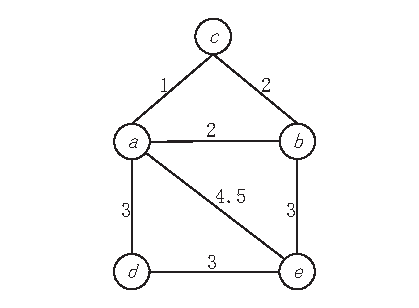
\includegraphics[width=0.5\columnwidth]{lfaexample}
\caption{Example for LFA}
\label{lfaexample}
\end{figure}


%LFC can protect against a single link failure, NPC can protect against a
%single node failure, while DC is applicable to more complex failure scenarios.
%We will now dive into the details of LFA.

\textbf{LFC:}
$x$ can be chosen when $C_x(d)\!<\!C_x(c)\!+\!C_{c}(d)$,
which means when packets are routed from $x$ to $d$, they will not be routed back to $c$,
since $C_{x}(c)+C_{c}(d)$ is the lowest cost of any path from $x$ to $d$ that passes $c$.
So the protection route will bypass $c$, thus bypass link $(c,b)$ too.

\textbf{NPC:}
$x$ can be chosen when $C_x(d)<C_x(b)+C_b(d)$,
which means the protection route will bypass $b$, thus also bypass link $(c,b)$.

\textbf{DC:}
$x$ can be chosen when $C_x(d)<C_c(d)$,
which means the protection route will bypass $c$ (and link $(c,b)$),
and the remaining cost to the destination strictly decreases.

From the explanation above, we can see all of the three criteria can bypass a link failure,
while \textbf{NPC} can also bypass a node failure.
In addition, \textbf{DC} has a nice property that even when used simultaneously by multiple nodes,
there will be no loop due to the decreasing cost to the destination,
while \textbf{LFC} and \textbf{NPC} can only be used by node $c$ locally.
This property makes \textbf{DC} useful in building multipath routing algorithms \cite{TBFH, dmpa, Yang_Source:2006}.


As in the concrete example of Fig. \ref{lfaexample}, let $c$ be the computing node.
For all packets destined to $d$,
$c$ selects node $b$ as its default next hop.
Since $C_a(d)=5, C_{a}(c)=2$, and $C_{c}(d)=4$, node $a$ satisfies \textbf{LFC}, i.e., $C_a(d)<C_a(c)+C_c(d)$,
and can be used as an alternate next hop if the link $(c,b)$ fails.
However, node $a$ does not satisfy \textbf{NPC} since $C_a(d)=C_a(b)+C_b(d)$,
so if the failed component is node $b$, $a$ cannot be used as an alternate.
Similarly, since $C_a(d)>C_c(d)$, $a$ cannot be used in \textbf{DC} based multipath routing schemes.

Now consider another destination $e$, and the default next hop on $c$ for destination $e$ will now be $a$.
Since $C_b(e)<C_b(c)+C_c(e)$, $C_b(e)<C_b(a)+C_a(e)$, and $C_{b}(e)<C_{c}(e)$,
$b$ is a valid next hop for destination $e$ according to anyone of \textbf{LFC}, \textbf{NPC}, and \textbf{DC},
so it can be used for local route protection from link failure and node failure,
and for \textbf{DC} based  multipath routing.


%Since the performance of routing and forwarding is critical to the Internet, routing protection algorithm has to be highly efficient to avoid becoming a bottleneck. However, the existing approaches often focus on finding more, or  disjoint paths, rather than reducing the computation or the communication overhead, which is the focus of this paper.

\iffalse In \cite{dmpa}, we propose a shortest path tree based multipath routing
algorithm called DMPA. DMPA guarantees loop-freeness of
the induced routing path by implicitly maintaining a partial
order of the routers underpinning it The time complexity of
DMPA does not depend on the degree of the calculating router.
However, the protection ration of DMPA is still lower than
the DC.
Unlike the above works, however, our main concerns are computational efficiency and network availability, as these are critical for the routing protection algorithm. Based on the existing work on this research area, we for the first time propose two routing protection algorithms (IAC and IAC) whose complexity is less than that of Dijkstra��s algorithm and also have a high network availability.

Unlike the above works, however, our main concerns
are computational efficiency and protection ratio, as these are
critical for the Algorithm. Based on the existing work on this
research area, we for the first time propose an algorithm whose
complexity is less than that of Dijkstras algorithm and without
degrading the protection ratio.
\fi

%Unlike the above works, however, our main concerns are computational efficiency and network availability, as these are critical for the routing protection algorithm. Based on the existing work on this research area, we for the first time propose a routing protection algorithm whose complexity is less than that of Dijkstra��s algorithm and also has a high network availability.

\iffalse
\section{Network Model}\label{model}
\begin{table*}[t]
\setlength{\belowcaptionskip}{0pt}
\normalsize
\caption{Notations}
\label{notation}
\centering
\begin{tabular}{c|c}
\hline
$G\!=\!(V,E)$&Undirected graph with nodes and edges\\
%\hline
%$V$&Set of nodes in the graph\\
%\hline
%$E$&Set of links in the graph\\
%\hline
%$R(v)$&Router-ID of node $v$\\
\hline
$L(u,v)$&Direct link cost between node $u$ and node $v$\\
\hline
$r(u,v)$&The link failure probability between node $u$ and node $v$\\
\hline
 $G'=G^w_{(u,v)}$  &The network topology when the edge
$(l,m)\in E$ change its weight to $w$\\
\hline
$T_c$&Shortest path tree rooted at node $c$\\
\hline
$T_{c}^{G'}$ &Shortest path tree rooted at node $c$ in $G'$ \\
\hline
$C_c(v)$ &The shortest cost from $c$ to $v$ in the original network$G\!=\!(V,E)$\\
\hline
$C_c^{G'}(d)$ &The shortest cost from node $c$  to node $d$ in the network $G'$\\
\hline
$N(v)$&Neighbors of node $v$\\
\hline
$D_c(v)$&Descendants of node $v$ (itself is included) in $T_c$\\
\hline
$D_c^{G'}(v)$&Descendants of node $v$ (itself is included) in $T_{c}^{G'}$\\
\hline
$N_{c}(v)$&Next-hop set computed by node $c$ for destination node $v$\\
\hline
$B_{c}(v)$&Best next-hop computed by node $c$ for destination node $v$\\

%\hline
%$p(v)$&tentative parent of $v$\\
%\hline
%$d(v)$&tentative cost from $c$ to $v$\\
\hline
\end{tabular}
\end{table*}

In this paper, we will limit our research to intra-domain link state routing protocols, e.g. OSPF and IS-IS. Each router in a single routing area maintains an identical network map which allows them to compute the shortest path to every other router in a routing area. Then each router construct its FIB table employing the above information. When a packet arrives at a router, a destination address based method is using to determine how to forward the packets to its corresponding interface. When the network topology changes, the routers adjacent to the changed component detects the change and then propagates the information to its neighboring router through the link state advertisement (LSA) information. After a period of time, all routers in this routing area are aware of  the change information and update their routing tables accordingly, then the network is at a stable state.


In the following sections, a network is modeled as a simple, undirected weighted graph $G=(V,E)$, where $V$ and $E$ respectively denote the set of nodes (routers) and the set of edges (links) in the network. Every link $(u,v)\in E$ in the network has an associated integer weight $L(u,v)$ and a failure probability $r(u,v)$. And the weights of the links in the network are symmetric.
$C_c(v)$ is the lowest cost from $c$ to $v$ in the network.
We use $N(v)$ to denote the neighbor set of the node $v$.
For a node $u\in N(V)$, we have $C_u(v)=C_v(u)=L(u,v)$.

In a link state routing network, the computing node $c$ builds a shortest path tree $T_c$ rooted at itself, containing
all the nodes in the network as potential destinations in the link state routing protocols, such as OSPF and IS-IS.
Then the router $c$ construct its FIB table based on the above information.
In particular, we use $B_{c}(v)$ to represent the best/default candidate,
which lies along the shortest path from $c$ to $v$.
Since $T_c$ is a shortest path tree, leading to the following lemma.
\begin{lemma} {\bf The Best Next-Hop Rule}
\label{bestnh}
\begin{equation}
B_c(v)=\begin{cases}
v&\mbox{$P_c(v)=c$}\\
B_c(P_c(v))&\mbox{$P_c(v)\neq c$}
\end{cases}
\end{equation}
\end{lemma}
Equation (\ref{bestnh}) in Lemma \ref{bestnh} means the best next-hop
$B_c(v)$ for a destination $v$ is $c$'s direct
child along the path from $c$ to $v$ in $T_c$.
A shortest path routing algorithm, such as open shortest path first (OSPF) \cite{moy1998rfc,moy1998ospf},
computes a single next-hop $B_{c}(v)$ by employing equation (\ref{bestnh})
at each step when a new node $v$ is added to the SPT.

We use $G'=(V,E,(l,m,w))$ to represent the new topology when the edge
$(l,m)\in E$ change its weight to $w$, $C_c(v,(l,m,w))$ is the shortest cost from node $c$  to node $v$ in the new network $G'=(V,E,(l,m,w))$.
$T_{c}(c,x,w)$ denote the new shortest path tree when the edge $(c,x)\in T_c$ change its weight to $w$.
For ease of reading, we summarize some  symbols in the Table \ref{notation}.

 $T_{c}$ represent a shortest path tree rooted at $c$, $D(T_{c},v)$ represent the descendants of node $v$ (node $v$ is excluded) in $T_{c}$,
$C_c(v)$ is the shortest cost from node $c$  to node $v$ in the original network $G$.
\fi




\section{Incremental Alternates Computation}\label{iac}
\iffalse
Given sets of nodes $N \in V$, $I(N)=\{S(e)\notin N, E(e) \in N\}$, $O(N)=\{S(e)\in N, E(e) \notin N\}$,
obviously $I(N)=O(N)$ in an undirected connected graph $G$.
\fi

\subsection{Basic Idea}
On a router $c$, we focuses on how to efficiently compute alternate next hops for each destination.
We would like to adopt the criterion of \textbf{LFC}, or \textbf{NPC}, or \textbf{DC},
 in Section \ref{criteria} for different scenarios.
By carefully investigating each criterion, we can see that the difficulty
lies in computing, for each destination $d$, the lowest cost from each neighbor $x$ to $d$ (i.e., $C_{x}(d)$),
with $C_{x}(b)$ just being a special case. All the other costs,
including $C_{c}(d), C_{b}(d)$ and $C_{x}(c)$, are already available
since $c$ always maintains a shortest path tree rooted at itself,
while $C_{b}(d)$ is just $C_{c}(d)-C_{c}(b)$, and $C_{x}(c)$ is just $C_{c}(x)$.

Typical LFA implementations of nowadays router vendors naively maintain a SPT for each neighbor $x$,
thus requires $O(k)$*\textbf{SPT} time and space, where \textbf{SPT} is the complexity of constructing a SPT
from scratch. For nodes with a large number of neighbors, this will become
a bottleneck. TBFH \cite{TBFH} and DMPA \cite{dmpa} accelerate the computation at the cost of
failure repair capability and route availability, since they each utilize a criteria that is more restrict than \textbf{DC}.
For example, DMPA adopts $C_{c}(u)-C_{c}(x)+L(u,d)<C_{c}(d)$, where $u$ is a descendant of $x$,
and the left-hand equation is provably no less than $C_{x}(d)$. Thus DMPA, as well as TBFH,
computes less alternate next hops than our IAC algorithm which strictly follows the criterion of \textbf{DC}.
In addition, DMPA and TBFH cannot be easily adapted to follow \textbf{NPC} while IAC's
unified framework can also handle \textbf{NPC}.



Our algorithm IAC is actually embedded in a dynamic shortest path tree (SPT) algorithm, which takes
a graph and the corresponding SPT as input, and performs incremental shortest path computation
with the sign of some specific link cost simply reversed, i.e., from $\ell$ to $-\ell$. During this specific
dynamic update process, the cost from each neighbor $x$ to each destination $d$ can be efficiently computed,
and the alternates can be computed exactly according to each LFA criterion, achieving high speed, low space and
good quality simultaneously.

\iffalse
Since each node independently computes its next-hops for all destinations,
in the rest of the paper, our algorithm will be
described with respect to a particular node $c$ that performs such
kind of computation.

We denote the cost of the path from $c$ to $v$ in $T_{c}$ by $C_{c}(v)$,
the children of $v$ in $T_c$ by $H_c(v)$,
the parent of $v$ in $T_c$ by $P_{c}(v)$,
and the descendants of $v$ in $T_c$ by $D_c(v)$, with $c$ itself included.
\fi
\iffalse
\begin{figure*}[b]
        \centering
        \begin{subfigure}[b]{0.32\textwidth}
                \centering
                \includegraphics{shortpathtree}
                \caption{$T_{c}$}
              \label{spttree}
        \end{subfigure}
        \begin{subfigure}[b]{0.32\textwidth}
                \centering
                \includegraphics{sachange}
                \caption{$T'_{c}$ when $L(c,a)=0$}
                \label{spttreechange1}
        \end{subfigure}
         \begin{subfigure}[b]{0.32\textwidth}
                \centering
                \includegraphics{sbchange}
                \caption{$T'_{c}$ when $L(c,b)=0$}
                \label{spttreechange2}
        \end{subfigure}
        \caption{An example for explaining some Theorems}
        \label{theoremexample}
\end{figure*}
\fi
%To compute a set $N_{c}(v)$ of next-hops for $v$, we start with
%a simple rule called downstream criterion (DC) \cite{incits8473iso} rule.

\iffalse
\begin{figure}[h]
\centering
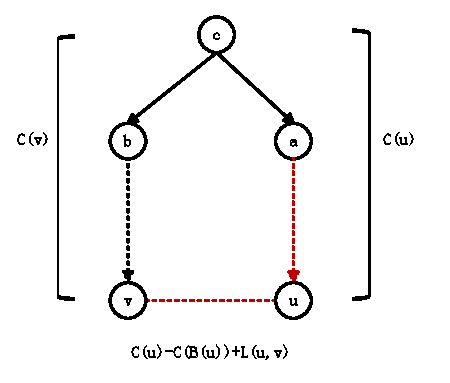
\includegraphics[width=3in]{proof}
\caption{Next-Hop contribution rule illustration}
\label{proofnh}
\end{figure}
\fi
\iffalse
\begin{figure}[t]
\centering
%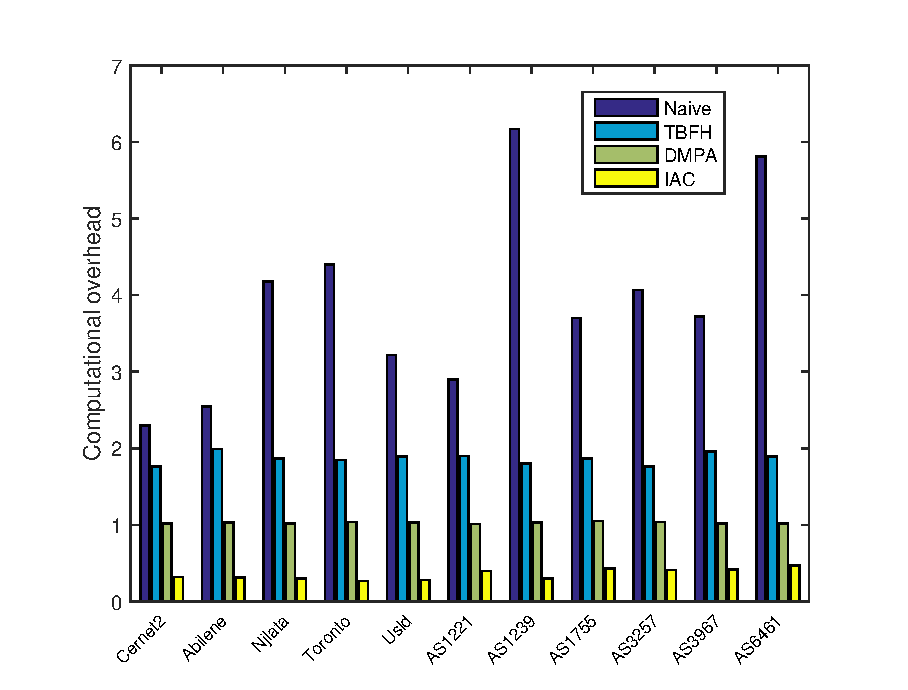
\includegraphics[width=3in]{realcomputationoverhead}
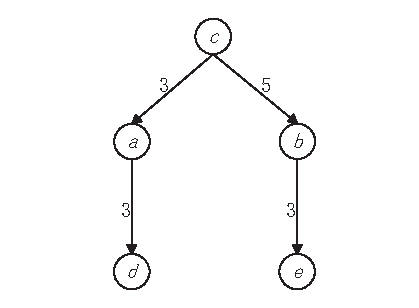
\includegraphics[width=2in]{dcspt}
\caption{Shortest path tree after link change}
\label{ispfspt}
\end{figure}
\begin{figure}[t]
\centering
%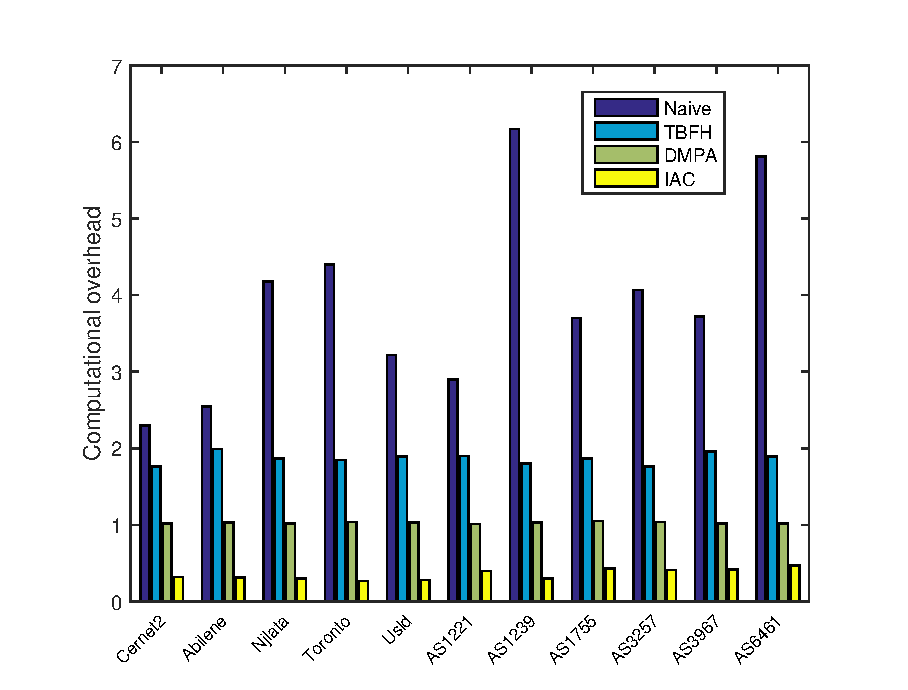
\includegraphics[width=3in]{realcomputationoverhead}
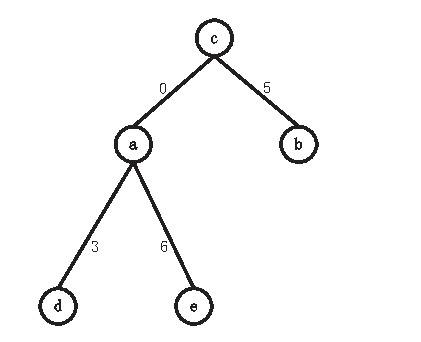
\includegraphics[width=2.5in]{dcsptcha1}
\caption{Shortest path tree after link change}
\label{ispfspt}
\end{figure}
\begin{figure}[t]
\centering
%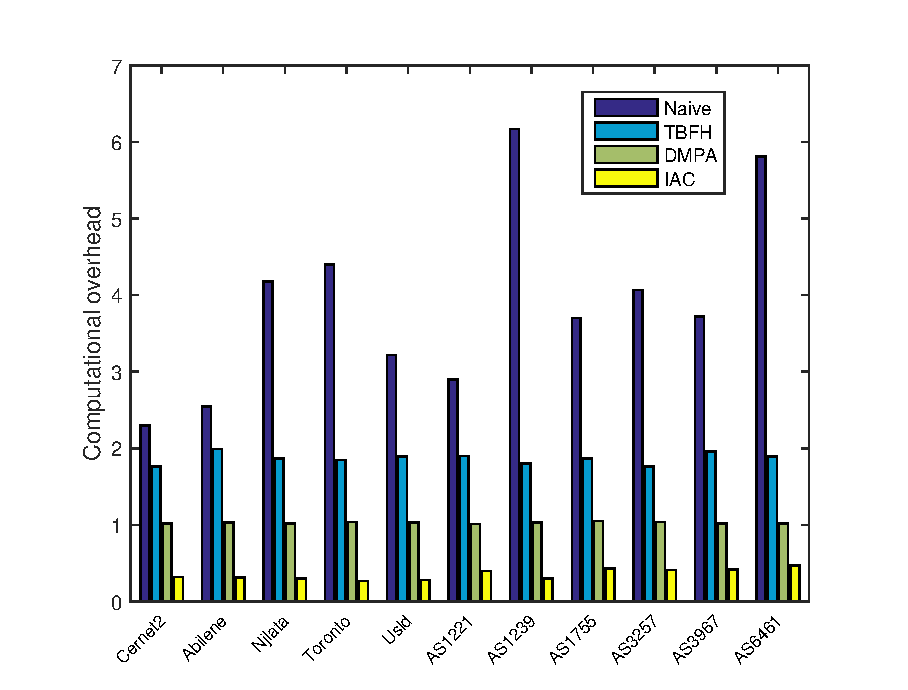
\includegraphics[width=3in]{realcomputationoverhead}
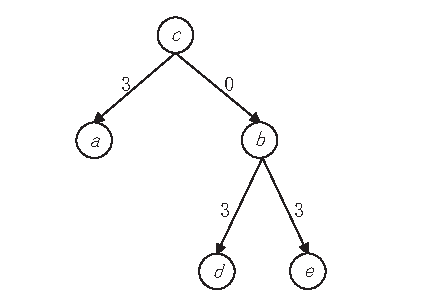
\includegraphics[width=2.5in]{dcsptcha2}
\caption{Shortest path tree after link change}
\label{ispfspt}
\end{figure}
\fi
\iffalse
\begin{theorem}\label{loop-free}
For packets destined to a destination $d$, if any node $c$ ($c \ne d$)
forwards them only to some nodes satisfy $C_v(d)<C_c(d)$,
there will be no loop in the network.
\end{theorem}
\begin{proof}
Consider a forwarding path $<v_{1}, v_{2}, ..., v_{k}, ...>$.
By the DC rule, we have $C_{(v_1)}(d) >C_{(v_2)}(d)$, $C_{(v_2)}(d) >C_{(v_3)}(d), ...$
$C_{(v_k)}(d) >C_{(v_(k+1))}(d)$, and so on. So there exists a strict partial order
between any two nodes on the path, and no node can appear twice on the
path, which means there is no loop.
\end{proof}
\fi
\iffalse
The DC rule is the basis of many loop-free multipath routing algorithms
\cite{Narvaez99efficientalgorithms, Yang_Source:2006, TBFH},
which differ in their ways to find such neighboring nodes that satisfy this rule.
\footnote{Their ways are also the root cause of their high complexity.}
\fi
\iffalse
In order to compute $C_v(d)$, it need to construct multiple
shortest path trees rooted at its neighbors,
so the induced cost will be particularly high for high degree nodes.
Therefore we propose a next-hop contribution rule in Theorem \ref {nhc},
which only need information of the local router.
\fi
\iffalse
If we naively compute $C_x(v)$ on node $c$ by constructing a SPT with $x$ as its root,
we will have to construct a SPT for each neighbor of $c$,
and the cost will be particularly high if the degree of $c$ is high.
The method will involve nontrivial computational overhead.
Such computation can consume a considerable
amount of CPU time, preventing other critical routing functions
from being executed. Thus, it is desirable to achieve this
using as little CPU time as possible.

For the actual deployment on the Internet, a LFA-based scheme should introduce a small additional burden on the current deployed routing protocol. This paper is dedicated to finding an efficient LFA-based scheme which is suitable for deploying on an ISP network. In particular, we focus on the following problem:
\textbf{\emph{Given a computing node $c$ and $T_c$, can we find an efficient LFA-based algorithmic technique and the algorithm conforms to the following two conditions:
(1)The time complexity of the algorithm is less than constructing a shortest path tree.
(2) It can provide the same protection ratio with LFA.
}}

\subsection{Algorithm Specification}
\iffalse
Before diving into the detail of IAC algorithm, we first describe DMPA.
DMPA propose a slightly more strict rule, \textbf{The Next-Hop Contribution Rule}, than the DC rule.

\begin{definition}
\label{selection}
Given any two nodes $u$ and $v$ in the shortest path tree $T_{c}$,
if
\begin{equation}
\label{nhc-eq}
C(u)-C(B(u))+L(u,v)<C(v),
\end{equation}
we say $u$ can contribute (the best next-hop for $u$) to (the next-hop set for) $v$.
\end{definition}



\iffalse
\begin{theorem} {\bf (The Next-Hop Contribution Rule)} \\
\label{nhc}
If $u$ can contribute to $v$, then $C_{B(u)}(v)\!<\!C(v)$,
and $c$ can use $B(u)$, the best next hop for $u$, as a next hop for $v$
without introducing forwarding loops.
%as suggested by the DC rule.
\end{theorem}
\fi
We will use an example to illustrate the Next-Hop contribution rule. In the Fig. \ref{proofnh},
$C(u)$ denote the cost of path $p=(c,a...,u)$ in the $T_c$,
$C(v)$ denote the cost of path $p=(c,b...,v)$ in the $T_c$,
$C(u)-C(B(u))+L(u,v)$ denote the cost of  path
$\lambda(p)\circ (u,v)$, where $\lambda(p)$ denote the subpath of $p$ from its second node to its last node and $\circ$ is the path concatenation operator.
We say $u$ can contribute to $v$
if $C(u)-C(B(u))+L(u,v)<C(v)$ is satisfied. Therefore, node $c$ can use $a$ as a validate next hop to $v$.
\iffalse
The merit of the next-hop contribution rule is that, it is very easy
to check whether inequality (\ref{nhc-eq}) can be satisfied for any two
nodes $u$ and $v$ in the SPT, since all terms in inequality (\ref{nhc-eq})
are known at that time.
So at each step when a new node $v$ is added to the SPT,
we can simply check whether any other node $u$ added earlier can contribute to it,
and add $B(u)$ to $N(v)$ if that is true. Similarly, if $v$ can contribute
to $u$, just add $B(v)$ to $N(u)$. In particular, we only need to do this
test if $u$ and $v$ are neighbors in the network, since otherwise $L(u,v)=\infty$
and (\ref{nhc-eq}) can never be satisfied. With this rule,
we can compute $N(v)$ for any node $v$ in a way faster than other multipath algorithms,
without introducing loops.
\fi
\begin{figure}[h]
\centering
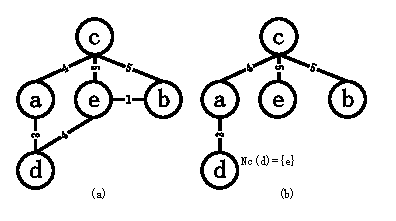
\includegraphics[width=3.8in]{mnpfexample}
\caption{An example for explaining the drawback of DMPA}
\label{drawback}
\end{figure}
Fig. \ref{drawback} gives an example to explain the drawback of DMPA.
Fig. \ref{drawback}(a) is a simple network topology  which consists of
5 node and 6 edges. Fig. \ref{drawback}(b) is a shortest path tree rooted at node $c$. From Fig. \ref{drawback}(b), we can get $C_b(d)=5<C_c(d)=7$, therefore
node $b$ is a feasible backup next-hop from $c$ to $d$. However, we cannot find this feasible backup next-hop employing DMPA. This drawback is due to that node $d$ only considers its neighbors' best next-hop as its potential backup next-hop.
The time complexity of DMPA does not depend on the degree of the calculating router. However, the network availability of DMPA is lower than that of the DC. Unlike the above work, DMPA, however, our main concerns are computational efficiency and network availability, as these are critical for the Algorithm. Based on the existing work on this research area, we for the first time propose an algorithm whose complexity is less than that of Dijkstra's algorithm and without degrading the  network availability of DC.
\label{algorithm}
We first provide two theorems before formally describing the details of the algorithm. The following two theorems describe how to compute all the DC backup next-hop set for node $c$. And the computation overhead can be dramatically reduced via reducing the times of the operation.
\fi


Our main concerns are computational efficiency and network availability, as these are critical for the Algorithm. Based on the existing work on this research area, we for the first time propose an algorithm whose complexity is less than that of Dijkstra's algorithm and without degrading the  network availability of LFA.

For any node $x\in N(c)$, if we can quickly calculate $C_x(v), v\in V$ in the $T_{c}$, then a efficient LFA-based method can be achieved. Therefore, the problem that needs to be solved in this paper can be described as follows: For any node $x\in N(c)$,  if $T_{c}$ it is given, whether could we find an efficient algorithm which can quickly compute $C_x(v), v\in V$ or not. Theorem \ref{computeneighborcost} answers how to solve the above problem and gives proof.



\fi


%\label{algorithm}







\iffalse
\begin{figure}[t]
\centering
\includegraphics[width=3in]{shortpathtree}
\caption{Computation Time for Real and Measured Topologies}
\label{ndavi}
\end{figure}
\begin{figure}[t]
\centering
\includegraphics[width=3in]{sachange}
\caption{Computation Time for Real and Measured Topologies}
\label{ndavi}
\end{figure}
\begin{figure}[t]
\centering
\includegraphics[width=3in]{sbchange}
\caption{Computation Time for Real and Measured Topologies}
\label{ndavi}
\end{figure}
\fi




\iffalse
\begin{figure}[h]
\centering
%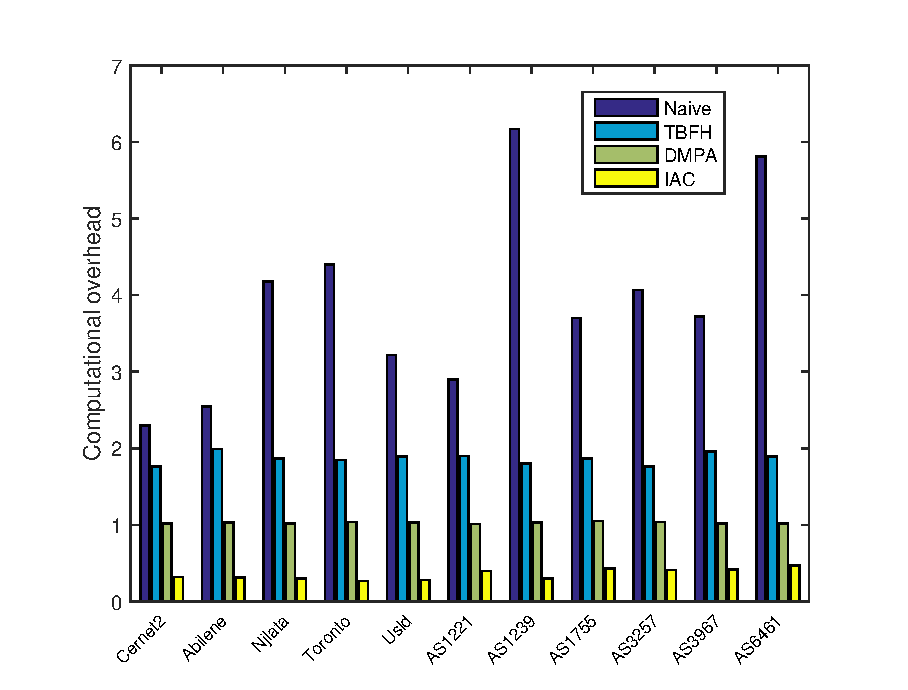
\includegraphics[width=3in]{realcomputationoverhead}
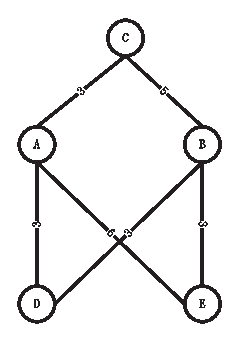
\includegraphics[width=3in]{dcnetworktopology}
\caption{Network topology}
\label{dcnetwork}
\end{figure}
\fi
\iffalse
We will use a simple example to explain the Theorem \ref{dcbackupnexthop}. Fig. \ref{dcnetwork} is a simple network work consists of  5 routers and 6 edges.
Fig. \ref{spttreedc} is a shortest path tree rooted at node $c$, while Fig. \ref{spttreechange1dc} and \ref{spttreechange2dc} respectively represent the new SPT when the weight of the links $(c,a)$  and $(c,b)$  is changed to $0$. Because $e \notin D(T_{c},a)$ and $e \in D(T'_{c},a)$, we can see that node $a$  can be a viable backup next-hop from   $c$ to $e$. Due to $d \notin D(T_{c},b)$, and $d \in D(T'_{c},b)$ ,  node $b$  can be a viable backup next-hop from $c$  to $d$, and also  we can get ode $b$  can be a viable backup next-hop from $c$  to $g$ in the same way.
\fi

\subsection{IAC Algorithm}
\begin{algorithm}[t]
\KwIn{Network graph $G=(V,E)$, the corresponding SPT $T_c$, and the LFA criterion}
\KwOut{$N_c(d)$  ($d \in V \backslash \{c\} $)}
%\SetAlgoNoLine
%\SetAlgoNoEnd
\ForEach{neighbor $x$ of $c$}{
make a temporary copy $T$ of $T_c$\;
\iffalse
\ForEach{$v \in V$}{
 %$v.visited \leftarrow floating$\;
 $C(v) \leftarrow C_c(v)$\;
% $P_{c}^{G_{(c,x)}}(v) \leftarrow P_c(v)$\;
}
\fi
%$c.visited=anchored$\;
 $weight\leftarrow L(c,x) $\;
 $L(c,x)\leftarrow -L(c,x)$\;
 %$newdist\leftarrow C_c(x)+\delta$\;
 %$\delta\leftarrow L(c,x)-weight$\;

 ENQUEUE$(\{x,(c,C_c(x)-2*L(c,x),-2*L(c,x)\})$\;
%\begin{shaded}
%\hl{(In IAC-NA $L(c,x)=-L(c,x)$)}\;
%\end{shaded}


 \iffalse
\For{$m\in D(T_c,x)$}
{
$C'_c(m)\leftarrow C'_c(m)-\delta$\;
%$m.visited=anchored$\;
}
\For{$v \in D(T_c,x)$}{
\For {each neighbor $u$ of $v$}{
\If {$u.visited=floating$ }
{
$newdist \leftarrow C_c(v)+L(v,u)$\;

\If {$newdist <C'_c(u)$}{
$\delta \leftarrow newdist-C'_c(u)$
ENQUEUE$(u,(v,newdist,\delta))$\;}
}
}
}
\fi
\While {$Q$ is not empty}{
$\{m,(p,n,\delta)\}\leftarrow$ EXTRACTMIN(Q)\;
%$P_c^{G_{(c,x)}}(m)\leftarrow n$\;
%$m.visited\leftarrow anchored$\;
adjust $T$ to make $p$ the parent of $m$\;
$C(m)\leftarrow n$\;
\ForEach{descendant $t$ of $m$}{
$C(t) \leftarrow C(t)+\delta$\;
}
\iffalse\ForEach{$d\in D_c(m)$}
{
$C_{c}^{G_{(c,x)}}(d)\leftarrow C_c(d)+\delta$\;

\If {$d \in D_c(x)$}
{$C_{x}(d)\leftarrow C_{c}(d)-C_{c}(x)$\;
}

\If {$d \notin D_c(x) \land d \in D_c^{G_{(c,x)}}(x)$}
{$C_{x}(d)\leftarrow C_{c}^{G_{(c,x)}}(d)+C_{c}(x)$\;
}
\If {$d \notin D_c(x) \land d \notin D_c^{G_{(c,x)}}(x)$}
{$C_{x}(d)\leftarrow C_{c}(d)+C_c(x)$\;
}

}
\fi
%Compute $C_x(v)$ using Theorem \ref{computeneighborcost}\;
%Add $x$ to $N_c(v)$;\quad\quad\quad\quad\quad\quad\quad\quad\quad\quad\quad\quad\quad\quad\quad\quad\quad\quad\quad
%\hl{(In IAC-NA Compute $C_x(v)$ using Theorem 9)} \;

\ForEach {neighbor $q$ of $m$}{
\If {$C_c(q)>C(m)+L(m,q)$ }
{

$newdist \leftarrow C(m)+L(m,q)$\;
$\delta\leftarrow newdist-C_c(q)$\;
ENQUEUE$(q,(m,newdist,\delta))$\;
}

}
}
 $L(c,x)\leftarrow weight$\;
%}
%\ForEach{neighbor $x$ of $c$}
%{
\ForEach{$d \in V\backslash \{c\}$}
{
\If {$d \in D_c(x)$}
{$C_{x}(d)\leftarrow C_{c}(d)-C_{c}(x)$\;
}

\If {$d \notin D_c(x)$ and $d$ is a descendant of $x$ in $T$}
{$C_{x}(d)\leftarrow C(d)+C_{c}(x)$\;
}
\If {$d \notin D_c(x)$ and $d$ is not a descendant of $x$ in $T$}
{$C_{x}(d)\leftarrow C_{c}(d)+C_c(x)$\;
}
\If {the LFA criterion is satisfied}
 {
 add $x$ to $N_c(d)$\;
 }
}
}
\Return $N_c(d) (d \in V \backslash \{c\})$
\caption{Incremental Alternates Computation}
\label{IAC-alg}
\end{algorithm}
\iffalse
\begin{figure*}[t]
\begin{subfigure}[b]{0.20\textwidth}
                \centering
                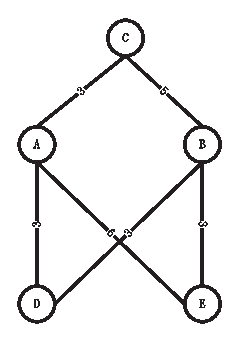
\includegraphics{dcnetworktopology}
                \caption{$T_{c}$}
              \label{dcnetwork}
        \end{subfigure}
        \begin{subfigure}[b]{0.24\textwidth}
                \centering
                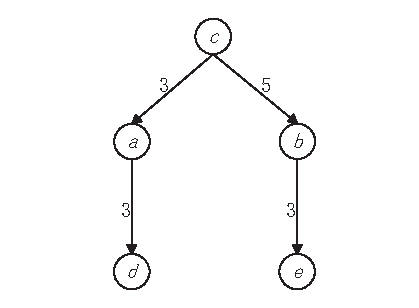
\includegraphics{dcspt}
                \caption{$T_{c}$}
              \label{spttreedc}
        \end{subfigure}
        \begin{subfigure}[b]{0.22\textwidth}
                \centering
                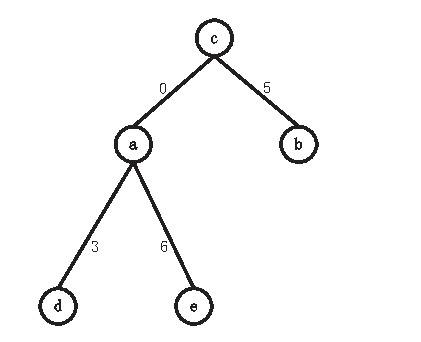
\includegraphics{dcsptcha1}
                \caption{$T_c(c,a,0)$}
                \label{spttreechange1dc}
        \end{subfigure}
         \begin{subfigure}[b]{0.24\textwidth}
                \centering
                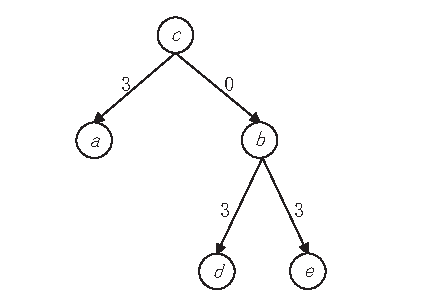
\includegraphics{dcsptcha2}
                \caption{$T_c(c,b,0)$}
                \label{spttreechange2dc}
        \end{subfigure}
        \caption{An example for explaining the Theorem \ref{dcbackupnexthop}}
        \label{theoremdc}
\end{figure*}
\fi

Algorithm \ref{IAC-alg} presents the pseudo code of IAC, where $C_{c}(*)$ and $D_{c}(*)$ denote,
for a give node, the lowest cost from $c$ to it in graph $G$, and its descendants
in the SPT $T_{c}^{G}$ (the superscript $G$ is omitted).
For each neighbor $x$ of $c$, IAC adopts the  ball-and-string model framework\cite{Narv2002New}
to perform an incremental shortest path tree construction for a specific link cost update,
i.e., cost of link $(c,x)$ is changed from $L(c,x)$ to $-L(c,x)$ (line 4).
In the framework, a priority queue $Q$ is maintained to determine the proper node whose
position in the new tree should be fixed.
Each element in $Q$ is of the form ${(u,(p,n,\delta))}$, where $p$ is the potential parent
for node $u$, $n$ denotes the potential lowest cost from $c$ to $u$,
and $\delta$ is the corresponding cost change. The incremental search begins by
inserting element $(x, (c, C_{c}(x)-2*L(c,x), -2*L(c,x)))$ in to the queue (line 5).
Then we extract the node $m$ with the lowest cost in $Q$ and fix its position as well as its descendants' positions, in the new tree (line 7 $\sim$ 8),
and update the cost from $c$ to these nodes (line 9 $\sim$ 11).
Note that here we use notation $C(*)$ without any subscript to keep track of the potential
lowest cost from $c$ to a node in the update process.
Then we search the potential lower costs of $m$'s neighbors, and insert them into $Q$
if the cost from the root $c$ can be reduced (line 13 $\sim$ 16) to allow further EXTRACTMIN operation.
Note that $m$'s descendants will not be reinserted into $Q$
since their costs and positions are already finalized.
After this incremental tree construction, we compute the cost from $x$ to each node,
and add the node to $N_{c}(d)$ if the LFA criterion is satisfied (line 18 $\sim$ 26).
Finally, after we complete this process for each neighbor of $c$, we return the set of
all alternate next hops for each destination $d$.

\iffalse
For any node $d$ in the network, the corresponding  $C_x(d)$ is computed
for

The $C_x(d)$
While compute the shortest cost $C_x(q)$ when the potential cost of $q$ is smaller than the old value (lines 26).
At last lines 28-31 are using to compute all the LFA next hop set for node $c$.
\fi
%\subsection{Example}


\begin{figure*}[t!]
        \centering
        \begin{subfigure}[b]{0.24\textwidth}
                \centering
                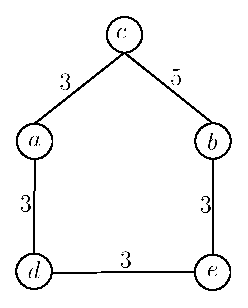
\includegraphics[width=0.8\textwidth]{nettopology}
                \caption{Network $G$}
              \label{spttree21}
        \end{subfigure}
        \begin{subfigure}[b]{0.24\textwidth}
                \centering
                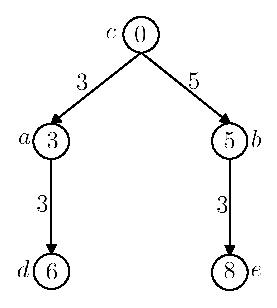
\includegraphics[width=0.8\textwidth]{sptc}
                \caption{$T_{c}$}
                \label{spttreechange22}
        \end{subfigure}
         \begin{subfigure}[b]{0.24\textwidth}
                \centering
                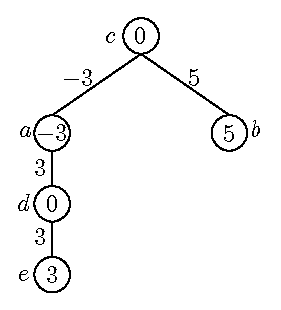
\includegraphics[width=0.8\textwidth]{newsptc}
                \caption{$T_{c}^{G_{(c,a)}}$}
                \label{spttreechange23}
        \end{subfigure}
         \begin{subfigure}[b]{0.24\textwidth}
                \centering
                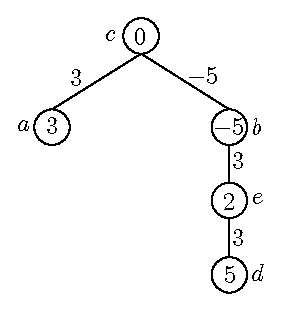
\includegraphics[width=0.8\textwidth]{newsptc1}
                \caption{$T_{c}^{G_{(c,b)}}$}
                \label{spttreechange24}
        \end{subfigure}
        \caption{An example for explaining how ICA works}
        \label{theoremexample}
\end{figure*}


Later, we will prove that this incremental tree construction process actually constructs the shortest path
tree for $G_{(c,x)}$, where $G_{(c,x)}$ is the dual graph of $G$ with the sign of $(c,x)$'s cost reversed,
and $C_{x}(d)$ is correctly computed. The proof has to be performed carefully, since the triangle
inequality property may not hold any more in the dual graph with negative link weight.

Before the formal proof, we use the following example to explain how ICA works.
Fig. \ref{spttree21} depicts a network topology consisting of 5 nodes and 6 edges, while the
corresponding SPT $T_{c}$ is depicted in Fig. \ref{spttreechange22}, with $c$ being the root.
For each neighbor or $c$, i.e., $a$ (or $b$), we use Algorithm \ref{IAC-alg} to compute a shortest path tree
$T_{c}^{G_{(c,a)}}$ (or $T_{c}^{G_{(c,b)}}$), where the sign of $(c,a)$'s (or $(c,b)$'s) cost is reversed.
The corresponding SPTs are depicted in Fig. \ref{spttreechange23} and Fig. \ref{spttreechange24}, respectively.

\iffalse
First, the node $a$ is enqueued into the $Q$ with its form \{$(a,(c,-3,-6))$\}.
In the first iteration, $(a,(c,-3,-6))$ will be selected.
The original subtree rooted at $a$  is considered together.
Therefore the node $d$ is selected at the same time.
Since $d$ has an outing edge to $e$, the potential cost and potential cost change of $e$ is calculated, which gives queue \{$(e,(e,3,-5))$\}. Node $d$ is selected in the next iteration.
The new shortest path tree rooted at $c$ is given in the
Fig. \ref{spttreechange23}.
\fi
For the neighbor $a$, according to line 19 $\sim$ 24 in Algorithm \ref{IAC-alg},
we compute the distance from each node to $a$ by:
\begin{align}
&C_a(d)=C_c(d)-C_c(a)=3,  \text{ since } d \in D_c(a) \nonumber\\
&C_a(e)=C(e)+C_c(a)=6,  \text{ since } e \notin D_c(a) \land e \in D_c^{G_{(c,a)}}(a) \nonumber\\
&C_a(b)=C_c(b)+C_c(a)=8,  \text{since } b \notin D_c(a) \land b \notin D_c^{G_{(c,a)}}(a) \nonumber
\end{align}
The correctness of this result, as well as the case for the neighbor $b$,
can be easily verified against the original topology.


\subsection{Theoretical  Analysis}
\iffalse
\begin{definition}
Given a shortest path tree $T_c$ and a network topology  $G'=G_{(c,x)}, (c,x)\in T_c$,
for any node $d\in V, d \neq c, d\in D_c(x)$,
we say the node $d$ change its position in $T_c^{G'}$, if and only if the
$d\in D_c^{G'}(x)$ is satisfied.
\end{definition}
\fi
\iffalse
\begin{theorem}\label{newspt0}
Given a shortest path tree $T_c$,
when the edge $(c,x)\in T_c$ change its weight to 0, the iSPF algorithm can get the correct new SPT $T_c(c,x,0)$.
\end{theorem}
\begin{proof}
The proof for this theorem is exactly the same as that of \cite{Narv2002New}, so the proof is omitted here.
\end{proof}
\begin{definition}
Given a shortest path tree $T_c$, we say a node $d$ change its position in $T_c(c,x,w)$, if and only if the shortest path from $c$ to $d$ is different in the  two trees.
\end{definition}
\begin{theorem}\label{newsptposition0}
Given a shortest path tree $T_c$, for any node $d(d\neq c, d\neq x)$, where $x \in N(c)$
\begin{itemize}
\item[(1)] If the position of the node $d$ in the new SPT $T_c(c,x,0)$ is  changed, then we have  $C_x(d)<C_c(d)$.
 \item[(2)] If $C_x(d)<C_c(d)$ is satisfied,  then the position of the node $d$ in the new SPT $T_c(c,x,0)$ will be changed.
\end{itemize}
\end{theorem}
\begin{proof}
(1)
If the position of the node $d$ in the new SPT $T_c(c,x,0)$ is changed, the node $d$ or its ancestor(s) must be enqueued into the $Q$ using ENQUEUE operation.
Assume that the difference between
the old cost and the potential new cost for the node $d$ is  $\delta$, the new shortest path cost of node $d$ is $C_c(d)-\delta$.
Since only the weight of the link $(c,x)$ is changed to 0, we have $d\in D(T_c(c,x,0),x)$. In $T_c(c,x,0)$, we have $C_c(d,(c,x,0))=C_c(x,(c,x,0))+C_x(d,(c,x,0))$.
Since $C_c(x,(c,x,0))=0$, we have $C_c(d,(c,x,0))=C_x(d,(c,x,0))$.
Because the shortest path from node $x$ to $d$ is not going through node $c$ in $T_c(c,x,0)$, we have $C_x(d,(c,x,0))=C_x(d)$.
Because $C_x(d,(c,x,0))=C_c(d)-\delta$,
we can get $C_x(d)=C_c(d)-\delta$.
Therefore, we have $C_x(d)<C_c(d)$.\\
(2)
Since $C_x(d)<C_c(d)$, the shortest path from node $c$ to node $d$ is not via node $c$.
When the weight of edge $(c,x)$ is changed from $L(c,x)$ to $0$, there exists a path $P=c,x,...,d$ from $c$ to $d$, and the cost of which is $C_c(x)+C_x(d)$.
Because $C_c(x)=0$, the cost of path $P$ is $C_x(d)$.
Therefore, the potential cost change for node $x$ is $C_c(d)-C_x(d)>0$.
The node $x$ will be enqueued into the $Q$ using ENQUEUE operation.
Since only the weight of the link $(c,x)$ is changed to 0, we have $d\in D(T_c(c,x,0),x)$. Therefore, the position of the node $d$ in the new SPT $T_c(c,x,0)$ will be changed.
\end{proof}
\fi
\iffalse
\begin{theorem}\label{newspttree0}
Given a $T_{c}$, $x \in N(c)$, for any node $d(d\neq c, d\neq x)$,
if the
\begin{itemize}
\item[(1)] if $d \notin D(T_{c},x)$ and $C_x(d)<C_c(d)$, then we have  $d\in D(T_c(c,x,0),x)$.
\item[(2)] if $d \notin D(T_{c},x)$ and $d \notin D(T_c(c,x,0),x)$, then we have $C_x(d)<C_c(d)$.
\end{itemize}
\end{theorem}
\begin{proof}

\end{proof}








We have already known that Dijkstra's algorithm \cite{Dijkstra1959A} is not applicable with the networks whose link have negative weights. From the above example, when the link $(c,a)$ change its weight to $-L(c,a)$, the correct new shortest path tree can be constructed using iSPF. Theorem \ref{newspt} indicates that this is not a special case.
\fi
In this section, we use the abbreviated notation $G'$ to represent the dual graph $G_{(c,x)}$ of $G$,
where the link cost of $(c,x)$ changes from $L(c,x)$ to $-L(c,x)$.
\begin{theorem}\label{newspt}
For each neighbor $x$ of node $c$, the dual graph $G'$ contains no negative cycle,
and Algorithm \ref{IAC-alg} constructs the corresponding SPT $T_{c}^{G'}$
and the lowest distance from $c$ to each node.
\end{theorem}
\begin{proof}
%the weight of the link $(c,x)$ is changed to $-L(c,x)$,
We prove by contradiction. Assume there exists a negative cycle in $G'=G_{(c,x)}$, then the cycle must go through $(c,x)$ since
it is the only link with negative cost, i.e., $-L(c,x)$ where $L(c,x)$ is the link cost in the prime graph $G$.
Let the cycle be $(c,x,y,...,c)$, and the lengths of the two paths
$(c,x)$ and $(x,y,...,c)$ in this cycle be $-L(c,x)$ and $Length(x,y,...,c)$ respectively,
then $-L(c,x)+Length(x,y,...,c)<0$. That means $Length(x,y,...,c)<L(c,x)$, which contradicts with our triangle inequality
assumption in $G$ that $L(c,x)$ is the lowest cost between $c$ and $x$.
Therefore, there must exist a SPT in $G'$, and the correctness of the tree construction procedure
in IAC can be proven by following the proof of the ball-and-string algorithm,
since IAC is just a special case with specifically crafted link cost decrease in their incremental
shortest tree algorithm\cite{Narv2002New}.
\iffalse
We will use inductive reasoning to prove this theorem.\\
(1)We first prove
the base case. When the weight of edge $(c,x)$ is changed from $L(c,x)$ to $-L(c,x)$.
The potential parent for node $x$ is $c$, the potential cost for node $x$ is $-L(c,x)$, the potential cost change for node $x$ is $-2*L(c,x)$. The node $x$ will be enqueued into the $Q$ using ENQUEUE operation. After this operation, the queue has one element in the form of
$(x,(c,-L(c,x),-2*L(c,x)))$. Because there is no node can decrease its cost by more than $-2*L(c,x)$. Therefore, all of the descendants of node $x$ will be  placed in the correct positions during the first iteration.\\
(2)The inductive step is the same as in the \cite{Narv2002New}, so we omitted the content.\fi
\end{proof}

\begin{theorem}\label{newsptd}
For $c$'s neighbor $x$ and any node $d$ that is $x$'s descendant in $T_c$,
$C_x(d)=C_c(d)-C_c(x)$.
\end{theorem}
\begin{proof}
Since the path from $x$ to $d$ in the SPT $T_c$ is also the shortest path from $x$ to $d$ in $G$,
$C_c(d)=C_c(x)+C_x(d)$. So we get $C_x(d)=C_c(d)-C_c(x)$.
\end{proof}

\begin{theorem}\label{newsptx}
For $c$'s neighbor $x$ and any node $d$ (other than $c$ and $x$) that is not $x$'s descendant in $T_c$, if
$d$ becomes $x$'s descendant in $T_{c}^{G'}$, then $C_x(d)=C_c^{G'}(d)+C_c(x)$. %$C_c^{G'}(d)=C_c^{G'}(x)+C_x(d)$.
\end{theorem}
\begin{proof}
Let $P$ denote the path from $x$ to $d$ in $T_{c}^{G'}$,
and let  $Length(P)$ denote the cost of $P$.
Let $Q$ denote the shortest path from $x$ to $d$ in $G$, and its cost is $C_x(d)$.
It is obvious that $Length(P) \ge C_{x}(d)$ since $P$ is also a path in $G$.
As $d$ is $x$'s descendant in SPT $T_c^{G'}$,
we know $(c,x) \notin P$, and  $C_c^{G'}(d)=C_c^{G'}(x)+Length(P)$.
Therefore $C_c^{G'}(d) \ge C_c^{G'}(x)+C_x(d)$.

Suppose $Q$ does not pass through $c$,
then we get a non-cycling path $(c,x) \oplus Q$ from $c$ to $d$ in $G'$,
whose path cost will be $C_c^{G'}(x)+C_x(d)$.
Since $C_c^{G'}(d)$ is the lowest cost from $c$ to $d$ in $G'$,
it cannot be larger than $C_c^{G'}(x)+C_x(d)$. Therefore, $C_c^{G'}(d)=C_c^{G'}(x)+C_x(d)$.

Suppose $Q$ passes through $c$,
then $C_x(d)=C_x(c)+C_c(d)$, therefore we get
$C_c^{G'}(d) \ge C_c^{G'}(x)+C_{x}(d) = C_c^{G'}(x)+C_x(c)+C_c(d)=-L(c,x)+L(c,x)+C_{c}(d)=C_{c}(d)$.
As $C_c^{G'}(d)$ can be no larger than $C_{c}(d)$, equality has to be achieved in the last inequation,
which means $C_c^{G'}(d)=C_c^{G'}(x)+C_x(d)$.
%and $Length(P)=C_{x}(d)$

As $C_c^{G'}(x)=-C_c(,x)$, we get $C_x(d)=C_c^{G'}(d)+C_c(x)$ in both conditions.
\end{proof}
\begin{theorem}\label{newsptposition}
For $c$'s neighbor $x$ and any node $d$ (other than $c$ and $x$) that is not $x$'s descendant in $T_c$,
$d$ becomes $x$'s descendant in $T_{c}^{G'}$ if and only if $C_x(d)<C_x(c)+C_c(d)$.
\end{theorem}
\begin{proof}
We first prove if $C_x(d)<C_x(c)+C_c(d)$, then  $d\in D_c^{G'}(x)$.
Since $C_x(d)<C_x(c)+C_c(d)$, the shortest path in $G$ from node $x$ to node $d$
does not pass through node $c$.
Let the path be denoted by $P(x,d)$, then we can construct a non-cycling path
$P(c,d)=(c,x) \oplus P(x,d)$ from $c$ to $d$ in $G_{(c,x)}$,
where $\oplus$ means the concatenation of two paths.
Since the link cost of $(c,x)$ in $G_{(c,x)}$ is $-L(c,x)$,
the cost of $P(c,d)$ in $G_{(c,x)}$ will be $-L(c,x)+C_x(d)$.
On the other hand, from the condition $C_x(d)<C_x(c)+C_c(d)$ we get $C_{x}(d)<L(c,x)+C_{c}(d)$,
which means $C_{c}(d)>-L(c,x)+C_{x}(d)$. Since $d$ is not a descendant of $x$ in $T_{c}$
(i.e., $d \notin D_c(x)$),
at some time, the condition of line 13 in Algorithm \ref{IAC-alg}
will be triggered, and $d$ will be inserted into $Q$ by the ENQUEUE operation in line 16,
and later positioned in the subtree rooted at $x$ as $x$'s descendant (i.e., $d \in D_c^{G'}(x)$).
From Theorem \ref{newspt}, we know the subtree is part of $T_{c}^{G_{(c,x)}}$.

We then prove if $d\in D_c^{G'}(x)$, then  $C_x(d)<C_x(c)+C_c(d)$.
According to Theorem \ref{newsptx}, we know $C_x(d)=C_c^{G'}(d)+L(c,x)$.
%Assume that the potential cost change for node $d$ is  $\delta$, the potential cost of node $d$ is $C_c(d)+\delta$.
%In $T_c^{G(c,x)}$, we have $C_c^{G(c,x)}(d)=C_c^{G(c,x)}(x)+C_x(d)$ according to Theorem \ref{newsptx}.
Since $d \notin D_c(x)$ and $d\in D_c^{G(c,x)}(x)$,
node $d$ must be inserted into the $Q$ by the ENQUEUE operation at some time,
while the cost $C_c^{G'}(d)$ must be less than $C_{c}(d)$ (line 13 in Algorithm \ref{IAC-alg}).
Thus $C_x(d)=C_c^{G'}(d)+L(c,x) < C_c(d)+L(c,x) = C_x(c)+C_c(d)$.
\end{proof}

\iffalse
Since , the shortest path from node $c$ to node $d$ is not via node $c$.
When the weight of edge $(c,x)$ is changed from $L(c,x)$ to $-L(c,x)$,
the potential cost change for node $d$ is $C_c(d)-C_x(d)+C_x(c)>0$.
The node $x$ will be enqueued into the $Q$ using ENQUEUE operation.
Since only the weight of the link $(c,x)$ is changed to $-L(c,x)$, we have $d\in D_c^{G'}(x)$.
\fi








\iffalse
\begin{theorem}
Given a $T_{c}$, $x \in N(c)$, for any node $d(d\neq c, d\neq x)$
\begin{itemize}
\item[(1)] if $v \notin D(T_{c},x)$ and $C_x(v)<C_c(v)+C_x(c)$, then we have  $v\in D(T_c(c,x,-L(c,x)),x)$.
\item[(2)] if $v \notin D(T_{c},x)$ and $C_x(v)=C_c(v)+C_x(c)$, then we have  $v\notin D(T_c(c,x,-L(c,x)),x)$.
\end{itemize}
\end{theorem}

\begin{theorem}\label{newsptposition1}
Given a $T_{c}$, $x \in N(c)$, for any node $d(d\neq c, d\neq x)$
\begin{itemize}
\item[(1)] If the position of the node $d$ in the new SPT $T_c(c,x,0)$ is  changed, then we have  $C_x(d)<C_c(d)+C_x(c)$.
\item[(2)] if $C_x(d)<C_c(d)+C_x(c)$ is satisfied,  then the position of the node $d$ in the new SPT $T_c(c,x,-L(c,x))$ is  changed.
\end{itemize}
\end{theorem}
\begin{proof}
\end{proof}
\begin{theorem}\label{newspttree1}
Given a $T_{c}$, $x \in N(c)$, for any node $v(v\neq c, v\neq x)$
\begin{itemize}
\item[(1)] if $v \notin D(T_{c},x)$ and $C_x(v)<C_c(v)+C_x(v)$, then we have  $v\in D(T_c(c,x,-L(c,x)),x)$.
\item[(2)] if $v \notin D(T_{c},x)$ and $v \notin D(T_c(c,x,-L(c,x)),x)$, then we have $C_x(v)<C_c(v)+C_x(v)$.
\end{itemize}
\end{theorem}
\begin{proof}
\end{proof}
\begin{lemma}\label{nochange}
For any node $m$ in the $G$, if $C_x(v)=C_c(v)+C_x(c)\geq C_c(m)$, the position of the node $m$ will be not changed in the new SPT $T_c(c,x,-L(c,x))$.
\end{lemma}
\begin{proof}
From theorem \ref{newspt}, we can easily get this lemma. Because $C_x(v)= C_c(v)+C_x(c)= C_c(m)$, the node $x$ will not be enqueued into the Queue.
\end{proof}
\begin{theorem}\label{newspttree}
Given a $T_{c}$, $x \in N(c)$, for any node $v(v\neq c, v\neq x)$
\begin{itemize}
\item[(1)] if $v \notin D(T_{c},x)$ and $C_x(v)<C_c(v)+C_x(c)$, then we have  $v\in D(T_c(c,x,-L(c,x)),x)$.
\item[(2)] if $v \notin D(T_{c},x)$ and $C_x(v)=C_c(v)+C_x(c)$, then we have  $v\notin D(T_c(c,x,-L(c,x)),x)$.
\end{itemize}
\end{theorem}
\begin{proof}
(1)We will prove the first part of this theorem  by contradiction. If  $v\notin D(T_c(c,x,-L(c,x)),x)$, from Lemma \ref{nochange} we have $C_x(v)\geq C_c(v)+C_x(c)$. This contradict the $C_x(v)<C_c(v)+C_x(c)$.\\
(2)From Lemma \ref{nochange} we can get the second part of this theorem is correct.
\end{proof}
\fi
%$v\in D(T_c(c,x,-L(c,x)),B_c(v))$,
\iffalse
From Theorem \ref{newsptposition}, we can see that if the shortest path from neighboring node $x$ to $d$ is not going through node $c$.
The node $d$  must be the descendant of node $x$ in the new shortest path tree when the  weight of $(c,x)$ is changed to $-L(c,x)$.
Contrarily, if the node $c$ is included in the shortest path from neighboring node $x$ to $d$. The node $d$  must not be the descendant of node $x$ in the new shortest path tree when the  weight of $(c,x)$ is changed to $-L(c,x)$.
\fi
\begin{theorem}\label{fan}
For $c$'s neighbor $x$ and any node $d$ (other than $c$ and $x$) that is not $x$'s descendant in $T_c$,
$d$ does not become $x$'s descendant in $T_{c}^{G'}$, then $C_x(d)=C_c(d)+C_c(x)$.
\end{theorem}
\begin{proof}
From Theorem \ref{newsptposition}, since $d \notin D_c(x)$ and $d \notin D_{c}^{G'}(x)$,
we have $C_x(d) \ge C_x(c)+C_c(d)$.
On the other hand, since $C_x(d)$ is the lowest cost from $x$ to $d$ in $G$,
$C_x(d) \le C_x(c)+C_c(d)$.
Combining these two inequalities, we get $C_x(d)=C_x(c)+C_c(d)=C_c(d)+C_c(x)$.
%Therefore, the lemma can be easily verified.
\end{proof}


\iffalse
\begin{theorem}\label{computeneighborcost}
Given a shortest path tree $T_c$ and a network topology  $G'=G_{(c,x)}, (c,x)\in T_c$, for any node $d (d\neq c \land d\neq x)$
\begin{itemize}
\item[(1)] if $d \in D_c(x)$, then we have $C_{x}(d)=C_{c}(d)-C_{c}(x)$.
\item[(2)] if $d \notin D_c(x)$ and $d \in D_c^{G'}(x)$, then we have
 $C_{x}(d)=C_{c}^{G'}(d)+C_{c}(x)$.
\item[(3)] if $d \notin D_c(x)$ and $d \notin D_c^{G'}(x)$, then we have
 $C_{x}(d)=C_{c}(d)+C_c(x)$.
\end{itemize}
\end{theorem}
\begin{proof}
(1) Since $d \in D_c(x)$, we have $C_{c}(d)=C_{c}(x)+C_{x}(d)$. Therefore, we can easy get $C_{x}(d)=C_{c}(d)-C_{c}(x)$.

(2) According to Theorem \ref{newsptx}, we have $C_{c}^{G'}(d)=C_{c}^{G'}(x)+C_{x}(d)$ if  $d \in D_c^{G'}(x)$.
Because $C_{c}^{G'}(x)=-C_c(x)$, we have
$C_{x}(d)=C_{c}^{G'}(d)+C_c(x)$.

(3) From lemma \ref{fan}, we have $C_{x}(d)=C_{c}(d)+C_c(x)$.
\end{proof}
\fi

\iffalse
\begin{theorem}\label{dcextend}
Given a computing node $c$ and $T_{c}$, for any node $x \in N(c)$ , $T'(c)$ is the new shortest path tree rooted at node $c$  when the weight of link $(c,x)$ is changed to 0. For any node $v(v\neq c, v\neq x)$, if $v \notin D(T_{c},x)$ and $v \in D(T'_{c},x)$, then we can get $C_{x}(v)<C_{c}(v)$.
\end{theorem}
\begin{proof}
Assuming that  $B_{c}(v)=y, y\neq x$ in the $T_{c}$, we have $C_{c}(v)=C_{c}(y)+C_{y}(v)$.
Since $v \in D(T'_{c},x)$, we can obtain $C'_{c}(v)=C_{c}(x)+C_{x}(v)$, where  $C'_{c}(v)$ is the cost from node $c$ to node $v$ in the $T'_{c}$. Because the weight of link $(c,x)$ in the $T'_{c}$ is 0, we can get  $C'_{c}(v)=C_{x}(v)$(1). According to that $v \notin D(T_{c},x)$ and $v \in D(T'_{c},x)$ , we can obtain $C'_{c}(v)<C_{c}(v)$  (2). Combining the equation (1) with (2), we have $C_{x}(v)<C_{c}(v)$.
\end{proof}
\fi
\iffalse
\begin{theorem}\label{dcbackupnexthop}
Given a shortest path tree $T_c$, for any node $d(d\neq c, d\neq x)$, if $d \notin D(T_{c},x)$ and $v \in D(T_{c}(c,x,0),x)$, then we can get $N_c(d)=N_c(d)\cup {x}$.
\end{theorem}
\begin{proof}
From the Theorem \ref{newspt0}, Theorem \ref{newsptposition0} and DC rule, we can see that the node   $x$ is a viable backup next-hop from node $c$ to node $d$, therefore we have $N_c(d)=N_c(d)\cup {x}$.
\end{proof}

\begin{theorem}\label{algorithmcorrect}
Given a shortest path tree $T_c$ and a network topology  $G'=G_{(c,x)}, (c,x)\in T_c$, the value of $C_x(d), d\neq c \land d\neq x$ can be correctly computed by IAC.
\end{theorem}
\begin{proof}
For any node $d\in T_c^{G'}$, the calculation of the value of $C_x(d)$ can be divided into three cases.

(1) If $d \in D_c(x)$, the lines 24-25 are executed.

(2)If $d \notin D_c(x) \land d \notin D_c^{G'}$, the lines 26-27 are executed.

(3)If $d \notin D_c(x) \land d \notin D_c^{G'}$, the lines 28-29 are executed.

According to Theorem \ref{computeneighborcost}, all of the $C_x(d), d \in V$ will be calculated when the lines ($23 \sim 29$) of the IAC are executed.
\end{proof}

\begin{theorem}\label{fullprooof}
Algorithm IAC can compute all the next hop set for node $c$ that satisfies the LFA Rule.
\end{theorem}
\begin{proof}
From Theorem \ref{algorithmcorrect}, all of the $C_x(d), d \in V$ will be calculated when the lines ($23 \sim 29$) of the IAC are executed.
As long as we know the above values, we can use the LFA rule to compute all the LFA next hop set for node $c$ (lines $30 \sim 31$).
\end{proof}
\fi



\iffalse
Now we will show the performance of the algorithm, including the time complexity and the number of backup next-hop computed by LFA. From theorem \ref{iaccomplexity}, we can see that the computational complexity of IAC is less than that of constructing a shortest path tree. From theorem \ref{fullprooof}, we can see that the IAC can compute all the backup next-hop set which satisfies the LFA Rule. We will describe the Theorem \ref{iaccomplexity} and Theorem \ref{fullprooof} in detail, and also their correctness is proved.
\fi

Incrementally constructing the SPT for the dual graph $G'$
and efficiently computing $C_x(d)$  for each $x$ and $d$ are
critical to IAC's correctness, completeness and efficiency.
Theorem \ref{newsptd}, Theorem \ref{newsptx} and Theorem \ref{fan} show concrete support
for line 19 $\sim$ 24 in Algorithm \ref{IAC-alg},
where $C_x(d)$ is computed in different ways for each situation.
%Next, we provide a simple analysis on IAC's complexity.

%\begin{theorem}\label{iaccomplexity}
%The computational complexity of IAC is less than $\lg|V|\sum_{i=1}^k{M_{i}}$ when the queue is implemented as a binary heap.
%\end{theorem}
%\begin{proof}
To compute all the backup next-hop sets on node $c$ for each destination in the network, 
IAC needs to run the incremental SPT construction (i.e., iSPF) algorithm $k$ times, 
where $k$ is the number of its neighbors.
For one neighbor $x$, let $\delta_{n}$ denote the number of potentially affected nodes, 
and $\delta_{e}$  the number of edges attached to one of these nodes. 
According to the ball-and-string model\cite{Narv2002New}, 
the worst case complexity of the iSPF procedure for this neighbor will be 
$O(\delta_{e}*lg(\delta_{n}))$ with a binary heap, or $O(\delta_{e}+\delta_{n}*lg(\delta_{n}))$ with a Fibonacci heap, 
The remaining part, including constructing the temporary tree and 
computing $C_{x}(d)$ for all destinations, requires only $O(|E|+|V|)$ time.

Therefore, the computational complexity of the Algorithm IAC is $\sum_{i=1}^k{M_{i}*lgN_{i}}.  \leq \lg|V|\sum_{i=1}^k{M_{i}}$.
Since $N_{i}<|V|$, the computational complexity of IAC is less than $\lg|V|\sum_{i=1}^k{M_{i}}$.

%The computational complexity in IAC for this neighbor $i$ can be expressed as $O(M_{i}lgN_{i})$ according to \ref{Narv2002New}.
%\end{proof}

\iffalse
\begin{theorem}\label{iacfullprooof}
Algorithm IAC can compute all the backup next-hop set that satisfies the LFA Rule.
\end{theorem}
\begin{proof}
We will prove the theorem by contradiction. Supposing that there is a node $d(d\neq c, d\neq x)$, $d \notin D(T_{c},x)$ and $C_x(d)<C_{c}(d)$, when the IAC is terminated. For any node $x \in N(c)$,
if $C_x(d)<C_{c}(d)$, we have $d \in D(T_{c},x)$ according to Theorem \ref{newspt0} and
Theorem \ref{newsptposition0}. This contradicts the assumption.
\end{proof}
\fi
\iffalse
\subsection{Discussions}
IAC algorithm can only handle DC rule. However, it cannot be directly applied to LFC and NPC rules. Therefore, IAC cannot completely solve LFA problem.
We want to ask whether we can find an general algorithm that can completely and efficiently solve LFA. We will discuss this issue in the following sections.
\fi
\iffalse
\subsection{Discussions}
In the following, we will discuss how to apply the INC algorithm to compute all the backup next-hop set which meets the LFC rule. The LFC can be expressed as follows:

For packets destined to a destination $v$, node $c$ ($c \ne v$)
can forward them to its neighboring node $x$ if
\begin{equation}\label{eqn-LFC}
C_x(v)<C_c(v)+C_c(x).
\end{equation}
The resulting paths are loop-free and will reach the destination.

The following two theorems describe how to compute all the LFC backup next-hop set for node $c$. And the computation overhead can be dramatically reduced via reducing the times of the operation.

\begin{theorem}\label{lfcextend}
Given a computing node $c$ and $T_{c}$, for any node $x \in N(c)$ , $T'(c)$ is the new shortest path tree rooted at node $c$  when the weight of link $(c,x)$ is changed to $-L(c,x)$. For any node $v(v\neq c, v\neq x)$, if $v \notin D(T_{c},x)$ and $v \in D(T'_{c},x)$, then we can get $C_{x}(v)<C_{c}(v)+C_{c}(x)$.
\end{theorem}
\begin{proof}
Assuming that  $B_{c}(v)=y, y\neq x$ in the $T_{c}$, we have $C_{c}(v)=C_{c}(y)+C_{y}(v)$.
Since $v \in D(T'_{c},x)$, we can obtain $C'_{c}(v)=C_{c}(x)+C_{x}(v)$, where  $C'_{c}(v)$ is the cost from node $c$ to node $v$ in the $T'_{c}$. Because the weight of link $(c,x)$ in the $T'_{c}$ is $-L(c,x)$, we can get  $C'_{c}(v)=C_{x}(v)-L(c,x)$(1). According to that $v \notin D(T_{c},x)$ and $v \in D(T'_{c},x)$ , we can obtain $C'_{c}(v)<C_{c}(v)$  (2). Combining the equation (1) with (2), we have $C_{x}(v)<C_{c}(v)+L(c,x)$. Because $C_{c}(x)=L(c,x)$, we can get $C_{x}(v)<C_{c}(v)+C_{c}(x)$.
\end{proof}
\begin{theorem}\label{lfcbackupnexthop}
Given a computing node $c$ and $T_{c}$, for any node $x \in N(c)$ , $T'(c)$ is the new shortest path tree rooted at node $c$  when the weight of link $(c,x)$ is changed to 0. For any node $v(v\neq c, v\neq x)$, if $v \notin D(T_{c},x)$ and $v \in D(T'_{c},x)$, then we can get $N_c(v)=N_c(v)\cup {x}$.
\end{theorem}
\begin{proof}
From the  Theorem \ref{lfcextend}
and LFC rule, we can see that the node   $x$ is a viable backup next-hop from node $c$ to node $v$, therefore we have $N_c(v)=N_c(v)\cup {x}$.
\end{proof}
In order to implement LFC, we only need to change the line 3 of the INC as  $L(c,x)\leftarrow -L(c,x)$. From Theorem \ref{mpnedccomplexity} and Theorem \ref{fulldcprooof}, we can also get the same conclusion that the computation complexity our algorithm is less than constructing a shortest path tree and can provide the same network availability with DC. Since the proofs of Theorem \ref{mpnedccomplexity} and \ref{fulldcprooof}  are similar
to those of \ref{mpnecomplexity} and \ref{fullprooof}, so we omitted them.
\begin{theorem}\label{mpnedccomplexity}
The computational complexity of INC is less than $O(|E|lg|V|)$ ��
\end{theorem}

\begin{theorem}\label{fulldcprooof}
Algorithm INC can compute all the backup next-hop set that satisfies the LFC Rule.
\end{theorem}

\fi












\iffalse

Since $N_n = |V|$ and $N_e = |E|$, Algorithm \ref{dijk}
costs at most $O(|V|)+O(N_{n}*\lg(N_{n})+N_{e}) = O(|V|*\lg(|V|)+|E|)$,
which is similar to the complexity of a full shortest path computation.



where $em_Q$ and $dk_Q$ are times needed to perform extract minimum and decrease key
operations in the $Q$, respectively.
Since there are at most $V$ nodes in the queue,
$T_e=O(1), T_{x}=\lg(N_n)$ and $T_{k}=O(1)$ when the queue is implemented as a Fibonacci heap \cite{knuth1977generalization},
and the total time is at most $O(N_n*\lg(N_{n})+N_e)$.

Since $N_n = |V|$ and $N_e = |E|$, Algorithm \ref{dijk}
costs at most $O(|V|)+O(N_{n}*\lg(N_{n})+N_{e}) = O(|V|*\lg(|V|)+|E|)$,
which is similar to the complexity of a full shortest path computation.


Because there are at most $|V|$ nodes in the $Q$,
a node is extracted from $Q$ and an edge is performed decrease key
takes $O(lg|V|)$ and $O(1)$ time complexity respectively
on Fibonacci heap \cite{knuth1977generalization}.

When a node is extracted from the queue, whose neighbors will be visited.
The unvisited neighbors have an \emph{Enqueue} operation, while the visited
neighbors and the node itself may have an \emph{Add} operation.
However, both of the functions have constant complexity.
Therefore, the complexity of Algorithm \ref{DMPA} is in $O(|V|lg|V|+|E|)$.


In this section, we will explain the time complexity of MPA in detail.
In order to maintain nodes, which need to be updated the positions (parents) and costs, we adopt a priority queue.
We define $N_{n}$ is the node number which must change their cost or parent attributes (or both),
and $N_{e}$ is the edge number that may cause any node in
the queue to change its cost (This is implemented by the decrease-key operation of the priority queue).
Assume the time needed by ENQUEUE to enqueue a node is $T_e$, the time
by EXTRACTMIN to extract the node with the minimum cost is $T_{x}$,
and the time by ENQUEUE (decrease-key) to update a node existing in the queue is $T_{k}$.
Since each of the $N_{n}$ nodes has to be enqueued and extracted exactly once,
and each of the $N_e$ edges can cause at most one decrease-key operation, the total queue operation time in all
execution of Algorithm \ref{dijk} is at most $O(N_{n}*T_{e}+N_{n}*T_{x}+N_{e}*T_{k})$.
Beside queue manipulations, some operations are called at most two times for each of the $N_e$ edges,
including modifying the next-hop sets,
while others are called at most once for each of the $N_n$ nodes to set their attributes.
Each of them can be completed in constant time (or constant amortized time), and  they cost $O(N_n+N_e)$ in total.
So the final time for all execution of Algorithm\ref{dijk} is still $O(N_{n}*T_{e}+N_{n}*T_{x}+N_{e}*T_{k})$.

Since there are at most $N_n$ nodes in the queue,
$T_e=O(1), T_{x}=\lg(N_n)$ and $T_{k}=O(1)$ when the queue is implemented as a Fibonacci heap \cite{knuth1977generalization},
and the total time is at most $O(N_n*\lg(N_{n})+N_e)$.

Since $N_n = |V|$ and $N_e = |E|$, Algorithm \ref{dijk}
costs at most $O(|V|)+O(N_{n}*\lg(N_{n})+N_{e}) = O(|V|*\lg(|V|)+|E|)$,
which is similar to the complexity of a full shortest path computation.
\fi

%\section{Incremental Alternate Computation with Negative Augmentation}\label{iacna}

\iffalse
\begin{figure}[t]
\centering
%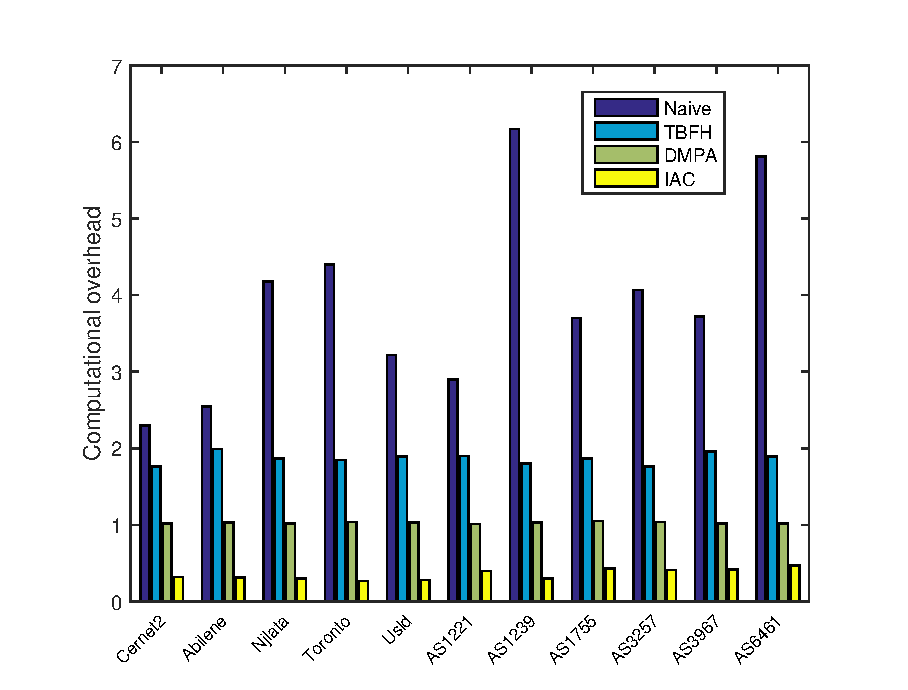
\includegraphics[width=3in]{realcomputationoverhead}
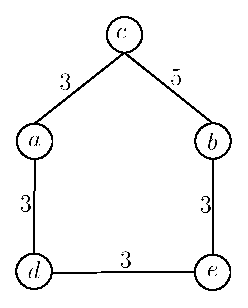
\includegraphics[width=2in]{nettopology}
\caption{network topology}
\label{realandrockettopologytime}
\end{figure}
\begin{figure}[t]
\centering
%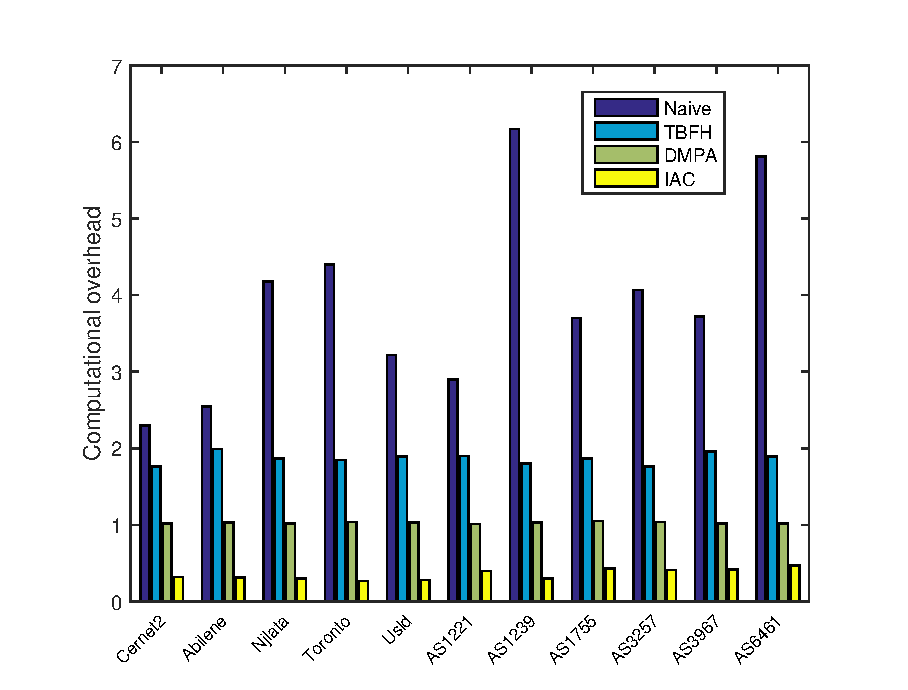
\includegraphics[width=3in]{realcomputationoverhead}
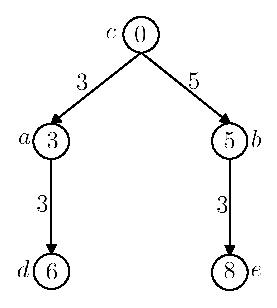
\includegraphics[width=2in]{sptc}
\caption{Shortest path tree rooted at node $c$}
\label{realandrockettopologytime}
\end{figure}
\begin{figure}[t]
\centering
%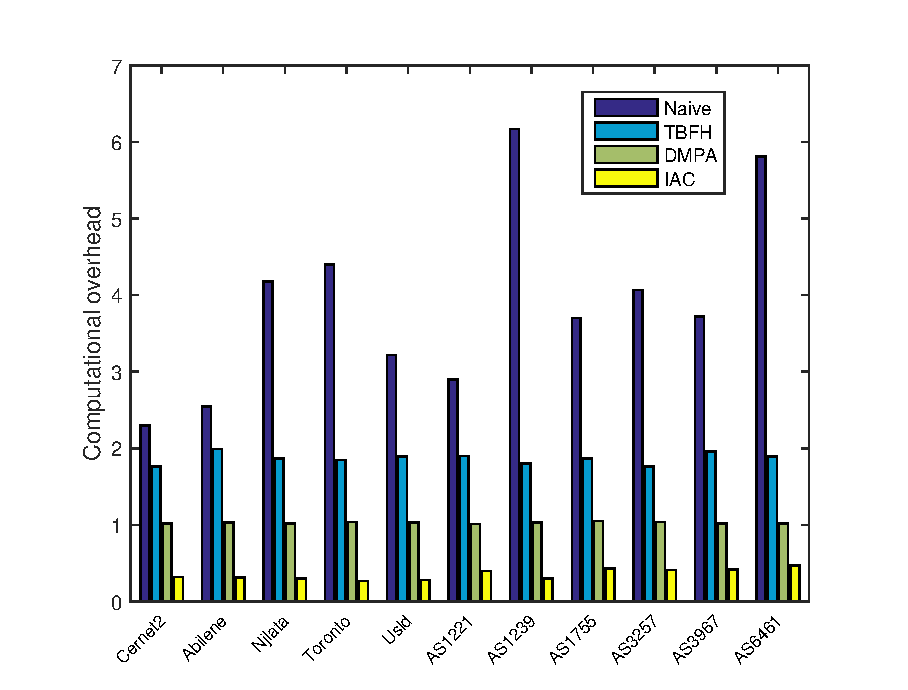
\includegraphics[width=3in]{realcomputationoverhead}
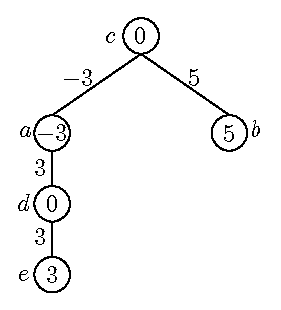
\includegraphics[width=2in]{newsptc}
\caption{New shortest path tree rooted at node $c$}
\label{realandrockettopologytime}
\end{figure}
\fi

\iffalse
\subsection{IAC-NC}
\iffalse
\begin{algorithm}[htb]
\KwIn{Network graph $G=(V,E)$}
\KwIn{$T_c$}
\KwOut{$N_c(v), (\forall v \in V \land v \neq c) $}
%\SetAlgoNoLine
%\SetAlgoNoEnd
\For{$x \in N(c)$}{
\For{$v \in V$}{
 $v.visited \leftarrow false$\;
 $C'_c(v) \leftarrow C_c(v)$\;
}
$c.visited=true$\;
 $weight\leftarrow L(c,x) $\;
 $L(c,x)\leftarrow -L(c,x)$\;

 $\delta\leftarrow weight-L(c,x)$\;
\For{$m\in D(T_c,x)$}
{
$C'_c(m)\leftarrow C'_c(m)-\delta$\;
$m.visited=true$\;
}
\For{$v \in D(T_c,x)$}{
\For {each neighbor $u$ of $v$}{
\If {$u.visited=false$ }
{
$newdist \leftarrow C'_c(v)+L(v,u)$\;
\If {$newdist <C'_c(u)$}{
ENQUEUE$(Q,(u,(v,newdist,\delta))$\;}
}
}
}

\While {$Q$ is not empty}{
$<v,tc> \leftarrow$ EXTRACTMIN(Q)\;

$v.visited\leftarrow true$\;
$C'_c(v)\leftarrow tc$\;

Compute $C_x(v)$ using Theorem \ref{computeneighborcost}\;
\For {each neighbor $u$ of $v$}{
\If {$u.visited=false$ }
{
$newdist \leftarrow C'_c(v)+L(v,u)$\;
\If {$newdist <C'_c(u)$}{
$\delta \leftarrow newdist-C'_c(u)$
ENQUEUE$(Q,(u,(v,newdist,\delta))$\;}
}
}
}
 $L(c,x)\leftarrow weight$\;
}
\For {$d\in V, d \neq c$}{
\For{$x\in N(c)$}
{
 \If {LFA is satisfied}
 {
 Add $x$ to $N_c(d)$\;
 }
}
}

\Return $N_c(v), (\forall v \in V \land v \neq c)$
\caption{IAC-NA}
\label{mnpe}
\end{algorithm}
\fi
Since the execution process of algorithm INC and INC-NA is basically similar, we will not repeat the same part in both of the algorithms.
Below, we will list the differences between the two algorithms. The line 7 in INC-NA is changed into $L(c,x)=-L(c,x)$. The line 22 in INC-NA is changed into Compute $C_x(v)$ using Theorem \ref{computeneighborcost}.
At last lines 29-32 are added to compute LFA next hop set for node $c$.
\fi
%However, for the completeness of the description, we still lists the pseudo code of the algorithm INC-NA.
%
\iffalse
We will elaborate the algorithm in detail in this section.
According to the above discussions, algorithm INC is proposed to compute the backup next-hop set which satisfies the DC rule. The inputs of the INC are the network topology $G=(V,E)$ and $T_{c}$, and the output is the backup next-hop set from node $c$ to all  other nodes in the network.
The INC requires several iterations. In each iteration,
at the beginning, the $visited$ attribute of all nodes except $c$ are set to $false$ (lines 2 $\sim$ 5). We change the weight of the link  $(c,x)$  to $-L(c,x)$, and compute the weight change for $(c,x)$ (lines 6 $\sim$ 8), which is  stored in variable $\delta$. The shortest cost from $c$ to $v$ and the $visited$ attribute of node $v$ are updated accordingly (lines 9 $\sim$ 11).
For $v \in D(T_c,x)$, for each of its unvisited neighbor $u$,
we compute the  new tentative cost  of $u$. The node $u$ will be inserted into
the $Q$ if its new tentative cost is smaller than the old value (lines 12 $\sim$ 17).
An $unvisited$ node $v$ with the lowest tentative cost will be popped out from the priority queue $Q$
by the EXTRACTMIN operation, where node ID is  used as tie breaking.
Then we can compute $C_x(v)$ using Theorem \ref{computeneighborcost}.
It is then added to the tree, marked as $visited$, and used as the $current\ node$ in the iteration,
while its attribute like cost  is also set to
a permanent value (lines $19 \sim 21$).
The corresponding node $x$ is added to the next-hop set $N_{c}(v)$
according to Theorem \ref{lfcbackupnexthop} (line 22).
For each unvisited neighbor $u$ of $v$,
we compute the  new tentative cost  of $u$. The node $u$ will be inserted into
the $Q$ if its new tentative cost is smaller than the old value (lines 23 $\sim$ 27).
At last, we will restore the weight of the link $(c,x)$ (line 28).
The LFA rule is used to calculate the backup next hop set from the node $c$ to all other nodes in the network.
\fi
%\subsection{Theoretical Analysis}
\iffalse
\begin{theorem}\label{mpnecomplexity}
The computational complexity of IAC-NA is less than $O(|E|lg|V|)$ when the queue is implemented as a Heap.
\end{theorem}
The proof for Theorem \ref{mpnecomplexity} is similar with that of Theorem \ref{iaccomplexity}, so we omit it.
\fi


\iffalse
\section{iSPF and LFA}\label{back}
In this section, we will discuss incremental shortest
path first (iSPF) algorithm and LFA, both of which are the foundation of our
work.
\subsection{Incremental Shortest Path First Algorithm}
The OSPF and IS-IS routing protocols which are
widely deployed in today��s Internet calculate a shortest path tree (SPT) from each router to other routers in an autonomous system (AS). Lots of commercial routers have adopted dynamic SPT algorithms which employ the structure of the previously computed SPT rather than recomputed an new SPT from scratch when the network topology changes. The reason is that when network topology changes, the new computed SPT does not differ conspicuously from the old one.

The incremental shortest path first algorithm (iSPF) maintains
a queue $Q$, each element in the queue is
of the form $(n,(p,d,\delta))$ , where $p$ denotes a potential parent
for node $n$, $d$ denotes a potential cost for node  $n$ , and $\delta$ denotes the potential cost change for node  $n$.
The  iSPF \cite{Narv2002New} is carried out as following steps:\\
(1)
Finding all the potentially affected nodes and marking them  \textsl{floating}.\\
(2) Computing the potential new cost, parent and the cost change $\delta$ between
the old cost and the potential new cost for the potentially affected nodes.\\
(3) In each iteration, a node with the smallest $\delta$ (least positive or most negative) is selected, and then a subtree, instead of only
one node, is appended to the new SPT. All of the above nodes are marked  \textsl{anchored}.
\begin{figure*}[t]
        \begin{subfigure}[b]{0.33\textwidth}
                \centering
                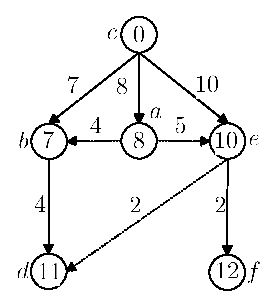
\includegraphics{ispfspt}
                \centering
                \caption{$T_{c}$}
              \label{spttree11}
        \end{subfigure}
        \begin{subfigure}[b]{0.33\textwidth}
                \centering
                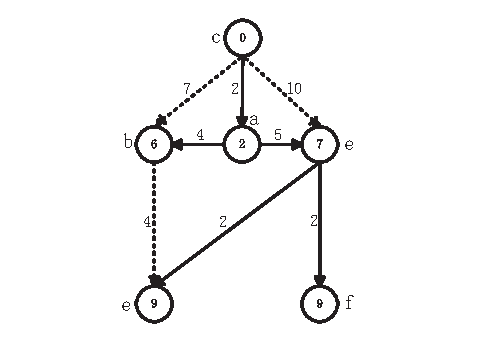
\includegraphics{ispfchange}
                \caption{shortest path tree when the $L(c,a)=2$}
                \label{spttreechange12}
        \end{subfigure}
         \begin{subfigure}[b]{0.33\textwidth}
                \centering
                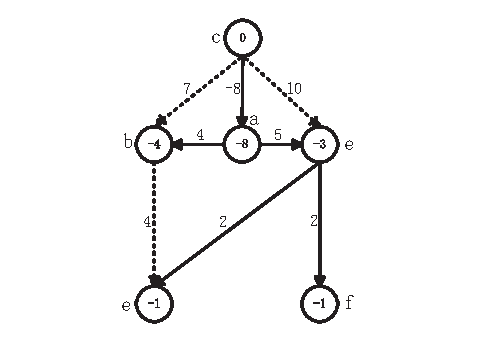
\includegraphics{ispfchange2}
                \caption{$T_{c}^{G_{(c,a)}}$}
                \label{spttreechange13}
        \end{subfigure}
        \caption{An example for explaining iSPF}
        \label{ex}
\end{figure*}
\iffalse
\begin{figure}[t]

\centering
%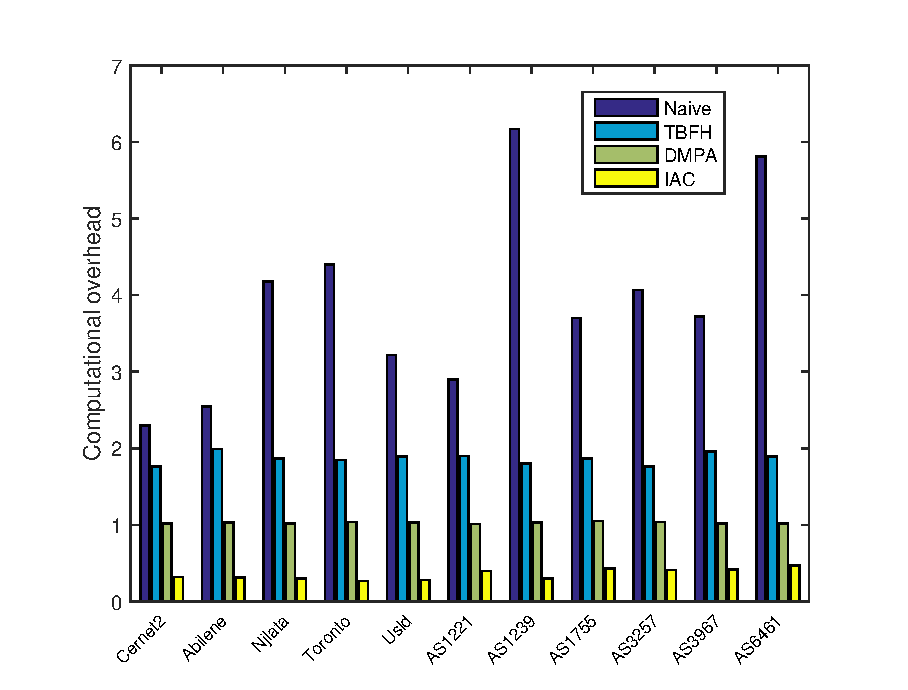
\includegraphics[width=3in]{realcomputationoverhead}
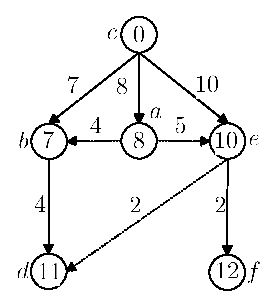
\includegraphics[width=3in]{ispfspt}
\caption{Shortest path tree rooted at $A$ before link change}
\label{ispfsptA}
\end{figure}
\begin{figure}[t]
\centering
%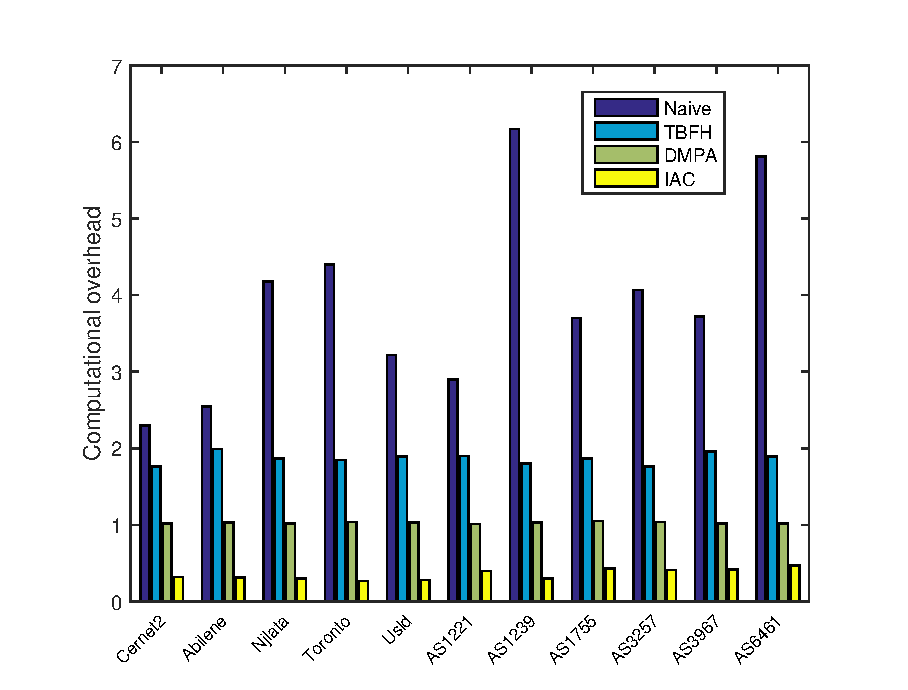
\includegraphics[width=3in]{realcomputationoverhead}
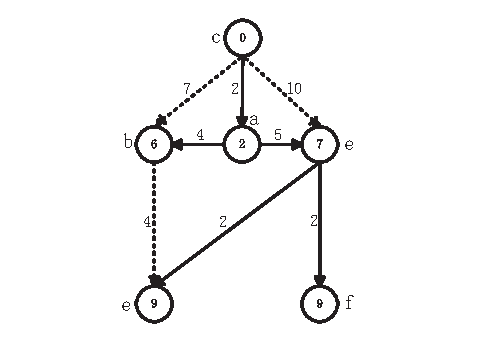
\includegraphics[width=3in]{ispfchange}
\caption{Shortest path tree rooted at $A$ when the weight of $(A,C)$ is changed to 2}
\label{ispfchangeA}
\end{figure}

\begin{figure}[t]
\centering
%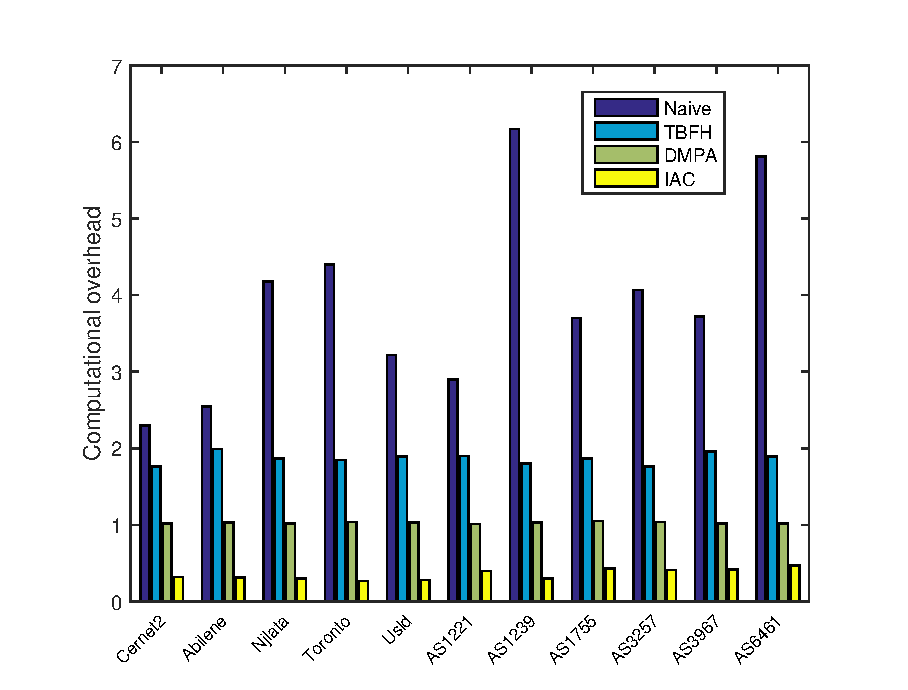
\includegraphics[width=3in]{realcomputationoverhead}
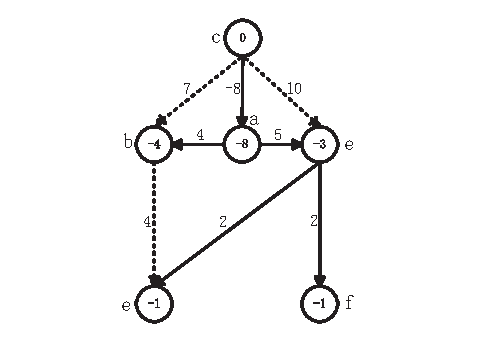
\includegraphics[width=3in]{ispfchange2}
\caption{Shortest path tree rooted at $A$ when the weight of $(A,C)$ is changed to -8}
\label{ispfchangeB}
\end{figure}
\fi

Perhaps the most intuitive way to demonstrate iSPF is through an
example. Consider the network topology depicted in Fig. \ref{spttree11}, which is composed of 6 nodes and 8 links. The letter besides the node is its label.
The solid lines are the links in the shortest path tree which is rooted at node $c$, while the dotted lines are the links  not in the above shortest path tree. The number inside the circle is the shortest cost from node $c$ to that node.

At some point, the weight of the edge $(c,a)$ is changed from 8 to 2.
Nodes except $c$ all affected nodes and are marked as \textsl{floating}.
Only the root node $c$ is marked as \textsl{anchored}. For all the \textsl{floating} nodes,
we check whether they have links to the \textsl{anchored} nodes, and calculate the new cost and the change  in cost. If the change in cost is smaller than 0, the node will be enqueued into the $Q$.
In the first iteration, the $Q$ has only one element with the form of
\{$(a,(c,2,-6))$\}.
In the next iteration, $(a,(c,2,6))$ will be selected and $a$ will be marked as \textsl{anchored}. Since $a$ has an outing edge to $e$ and $b$, the new cost and $\delta$ of $b$ and $e$ is calculated, which gives queue \{$(b,(a,6,-1)),(e,(a,7,-3))$\}. Then $e$ is selected, instead of only marking $e$ as \textsl{anchored}, the original subtree rooted at $e$  is considered together. Therefore the node $f$ is selected and marked as \textsl{anchored} at the same time. Since $e$ has an outing edge to $d$, the new cost and $\delta$ of $d$ is calculated, which gives queue \{$(b,(a,6,-1)),(d,(e,9,-2))$\}. Since node $d$ has the
largest potential shortest cost decrease, node $d$ is marked as \textsl{anchored}.
In the next iteration, node $b$ is selected.
The new shortest path tree is depicted in the
Fig. \ref{spttreechange12}.


Here we will describe a special example, when a single link changes its weight to the opposite number. For example, the weight of the edge $(c,a)$ is changed from 8 to -8. Only the root node $c$ is marked as anchored. For all the floating nodes,
we check whether they have links to the anchored nodes, and calculate the new cost and the change in cost, which gives
queue \{$(a,(c,2,-16))$\}.
In the next iteration, $(a,(c,2,-16))$ will be selected and  $a$ will be marked as anchored. Since $a$ has an outing edge to $e$ and $b$, the new cost and $\delta$ of $e$ and $b$ is calculated, which gives queue \{$(a,(b,-4,-11)),(e,(a,-3,-13))$\}. Then $e$ is selected, instead of only marking $e$ as anchored, the original subtree rooted at $e$  is considered together. Therefore the node $f$ is selected and marked as anchored at the same time. Since $e$ has an outing edge to $d$, the new cost and $\delta$ of $d$ is calculated, which gives queue \{$(a,(b,-4,-11)),(d,(e,-1,-12))$\}. Since node $d$ has the
largest potential shortest cost decrease, node $d$ is marked as anchored.
In the next iteration, node $b$ is selected.
The new shortest path tree is given in the
Fig. \ref{spttreechange13}.
\subsection{Some properties of the iSPF}
\fi

\section{Performance Evaluation}\label{evaluation}
Since our main motivation is to achieve good computational efficiency and LFA coverage,
we compare IAC with TBFH, DMPA, and the naive method that computes $k$ SPT.
Table \ref{britetable1} lists their capabilities of computing alternate next hops 
with respect to each criterion,
where ``$full$'' means the corresponding algorithm can compute all alternate next hops
that satisfy the LFA criterion in the column header, ``$partial$'' means only a subset
of alternate next hops for the criterion can be computed, while ``$-$'' means the algorithm
cannot be used for that criterion.  IAC and the naive method support all the three criteria and 
computes all the next hops. 
DMPA and TBFH, on the other hand, can compute a subset of next hops for \textbf{LFC}
and \textbf{DC} only.



\begin{table}[h]
\caption{Comparison of Different Algorithms}
\label{britetable1}
\centering
%\large
\normalsize
\begin{tabular}{|c|c|c|c|c|c|c|}% ͨ������ | ����ʾ�Ƿ���Ҫ��������
\hline  % �ڱ������Ϸ����ƺ���
Algorithm&LFC&NPC&DC\\
\hline
Naive&$full$&$full$&$full$\\
\hline
DMPA&$partial$&$-$&$partial$\\
\hline
TBFH&$partial$&$-$&$partial$\\
\hline % �ڱ������·����ƺ���
IAC&$full$ &$full$&$full$\\
\hline % �ڱ������·����ƺ���
\end{tabular}

\end{table}




\iffalse
Evaluation studies \cite{Gjoka2007Evaluation,Menth20101300} show that LFA protects against
many more failures than ECMP. Nevertheless, they also reveal that, on
average, LFA offers protection against only about 50\%
of all possible link failures and less than 40\% of node failures
Despite the limited protection it achieves, LFA is already supported by some equipment vendors \cite{cisco,Juniper}. With that in mind,
Retvari et al. \cite{lfarevisited} suggested that networks should be augmented with additional links to ensure that LFA can provide recovery
for all possible failures.
Therefore, our algorithms can directly use the above research findings, so that they can protect all single network component failure scenarios in the network.
\fi

We evaluate the performance of these algorithms in the following three types of topologies:
\begin{itemize}
\item [(1)] Topologies of real ISP networks, including CERNET2, Abilene, Njlata, Toronto, and Usld.
\item [(2)] Network topologies inferred by measurement studies\cite{2004148100061}, 
including AS1221, AS1239, AS1755, AS3257, AS3967, and AS6461. 
\item [(3)] Synthetic topologies generated by a random graph generator BRITE\cite{medina2001brite}. 
\end{itemize}

The topology size of the real and Inferred topologies varies from 11 to to 315, 
and the average node degree varies from 1.14 to 3.09, while in the synthetic topologies, 
the size and degree are set to be from 20 to 200, and from 5 to 25, respectively.
We note that a much larger node degree exists in practice,
i.e., there exit routes with even hundreds of neighbors,
but our evaluation on the topologies described above are already enough to demonstrate 
the gap between IAC and the other algorithms. 

\iffalse
Cernet2 (14 nodes, 16 links), Abilene (11 nodes, 14 links), Njlata (11 nodes, 23 links), Toronto (25 nodes, 55 links) and
Usld (28 nodes, 45 links)
and five ISP topologies which are measured by Rocketfuel\cite{2004148100061},
including   AS1221 (108 nodes, 153 links),
AS1239 (315 nodes, 972 links),
AS1755 (87 nodes, 161 links), AS3257 (161 nodes, 328 links),
AS3967 (79 nodes, 147 links), and AS6461  (128 nodes, 372 links) .
We also generate synthetic topologies with BRITE \cite{medina2001brite}.
The model is set to Waxman, mode is set to be Router only. The bandwidth
on each link follows a heavy-tail distribution ranging from
100 to 1024 \cite {Gjoka2007Evaluation} and the link cost is an inverse function of the bandwidth.
The parameters $\alpha$ and $\beta$ are set to 0.5.
%using parameters as listed in Table \ref{britetable}.
%In this section, we first show how link failures are modeled in our evaluation.

For similarity, we use a simple model to characterize link failure events.
The fail probability of each link $e$
is randomly generated in the range from 0 to 0.001.
All the simulations are conducted on a PC with Intel
i5 CPU, 1.7GHz and 1.5G Memory.

Due to space
constraints, we only present the results
for DC rule in the experiment, while the results for LFC and NPC
are similar.
\fi
%Because neither DMPA nor TBFH can implement the NPC rule,  so in the experiment we only compare the performance of the four methods on achieving  DC rule.

%Due to space constraints, we only list data for DC rules.
%Because neither DMPA nor TBFH can implement the NPC rule, IAC can only implement DC rule, so in the experiment we only compare the performance of
%the four methods on achieving  DC rule.

%Because IAC and IAC-NA have similar performance in realizing DC rule, IAC/IAC-NA is used to represent these two algorithms in the following section.
%In the following section, we will use IAC/IAC-NA to denote the IAC and IAC-NA.
\iffalse
\begin{table}[h]
%% increase table row spacing, adjust to taste
\normalsize
\renewcommand{\arraystretch}{1}
\caption{Parameters for BRITE}
\label{britetable}
\begin{center}
\begin{tabular}{c|c|c|c}
\hline
Model& N &   HS & LS  \\
\hline
Waxman & 20-1000&1000&100\\
\hline
\hline
m&NodePlacement &GrowthTypem & ${alpha}$  \\
\hline
2-40 & Random&Incremental&0.5\\
\hline
\hline
 ${beta}$ & BWDist &BwMin &BwMax \\
 \hline
0.5&Heavy Tail&100.0&1024.0\\
\hline
\end{tabular}
\end{center}
\end{table}
\fi
\subsection{Computation overhead}
\begin{figure*}[t!]
        \centering
        \begin{subfigure}[b]{0.32\textwidth}
                \centering
                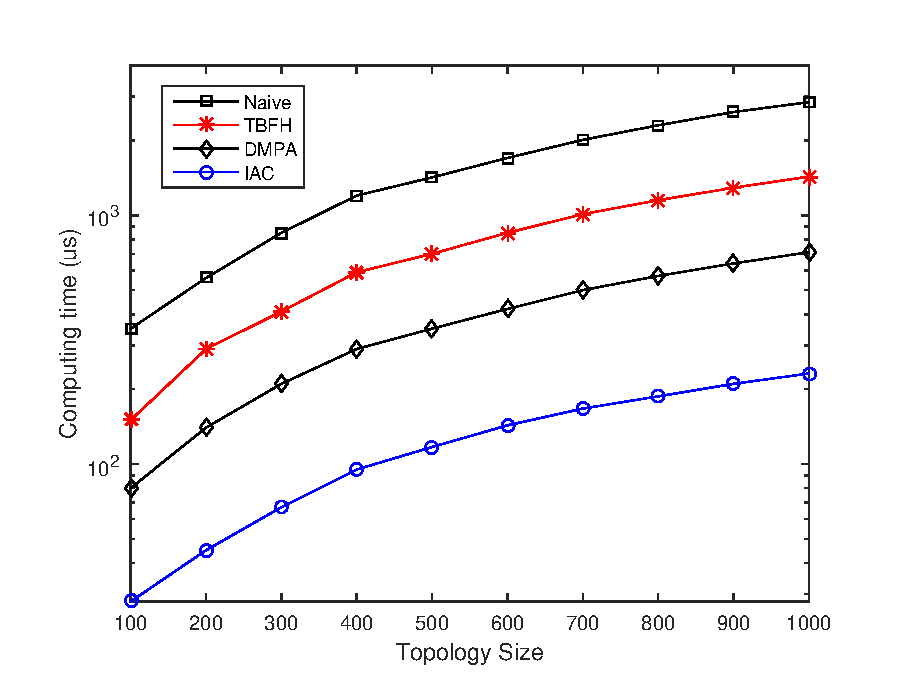
\includegraphics[width=\textwidth]{topcomputationoverhead}
                \caption{Varying topology size in Brite topologies}
              \label{topcom}
        \end{subfigure}
        \begin{subfigure}[b]{0.32\textwidth}
                \centering
                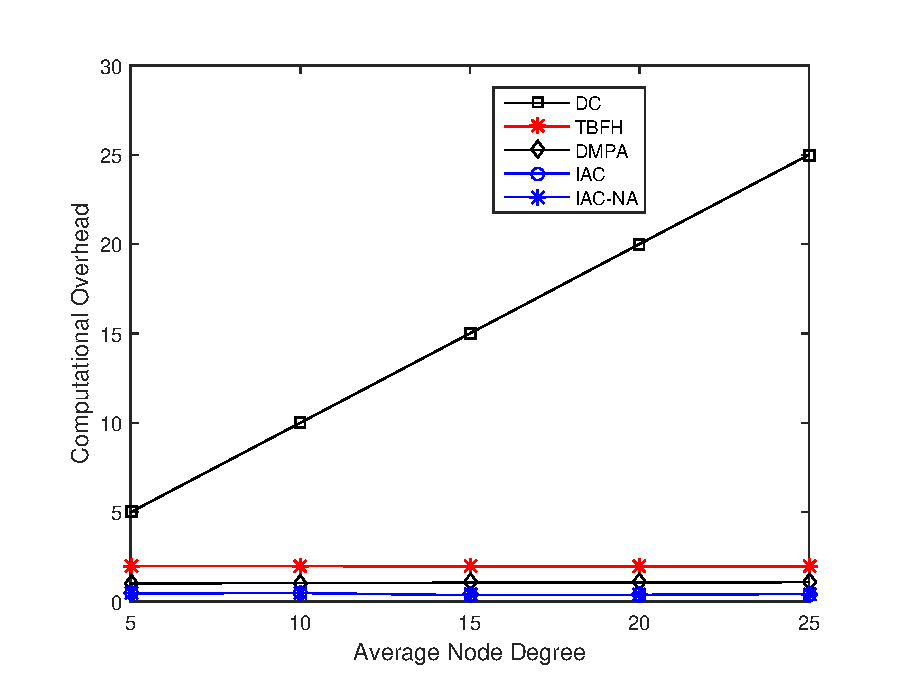
\includegraphics[width=\textwidth]{degcomputationoverhead}
                \caption{Varying node degree in Brite topologies}
                \label{nodedegreecom}
        \end{subfigure}
         \begin{subfigure}[b]{0.32\textwidth}
                \centering
                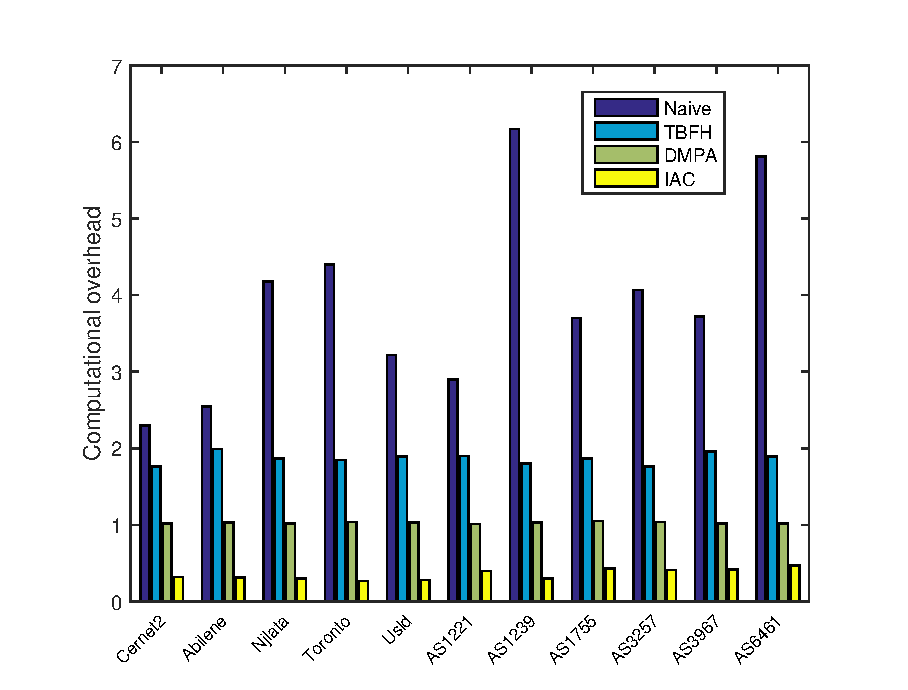
\includegraphics[width=\textwidth]{realcomputationoverhead}
                \caption{In real network topologies}
                \label{realtopologytime}
        \end{subfigure}
        \caption{Comparison on the computation complexity in different topologies}
        \label{comoverhead}
\end{figure*}


\begin{figure*}[t!]
        \centering
        \begin{subfigure}[b]{0.32\textwidth}
                \centering
                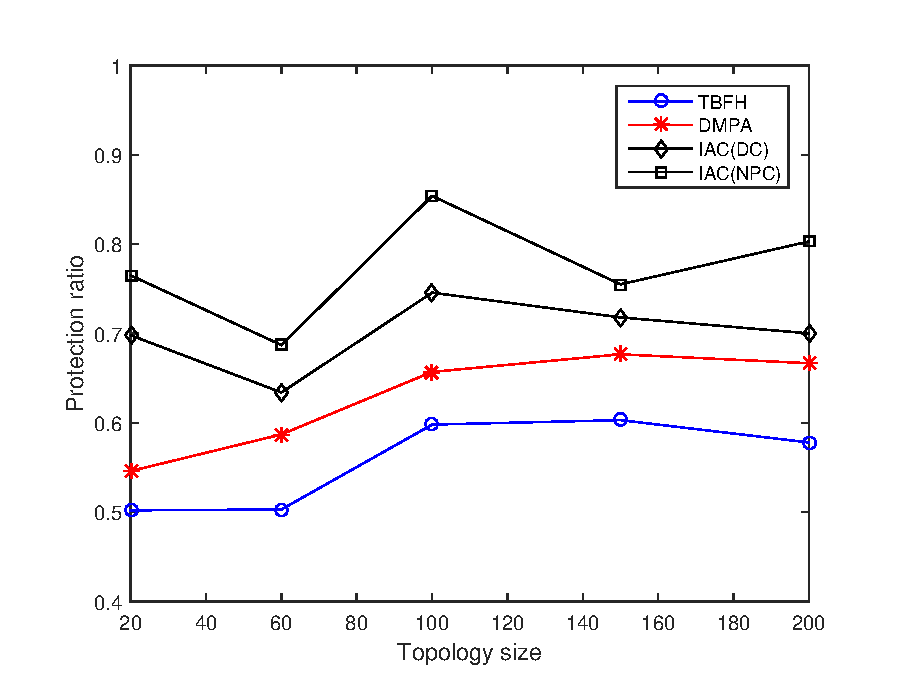
\includegraphics[width=\textwidth]{protectionratiotop}
                \caption{Varying topology size in Brite topologies}
              \label{prtop}
        \end{subfigure}
                 \begin{subfigure}[b]{0.32\textwidth}
                \centering
                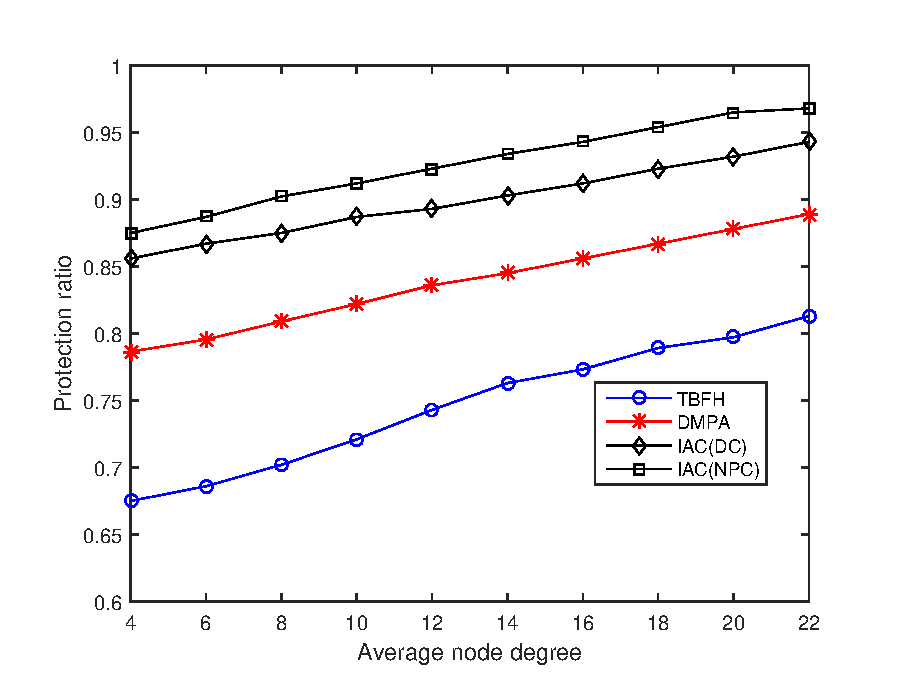
\includegraphics[width=\textwidth]{protectionratiodegree}
                \caption{Varying node degree in Brite topologies}
                \label{prd}
        \end{subfigure}
         \begin{subfigure}[b]{0.32\textwidth}
                \centering
                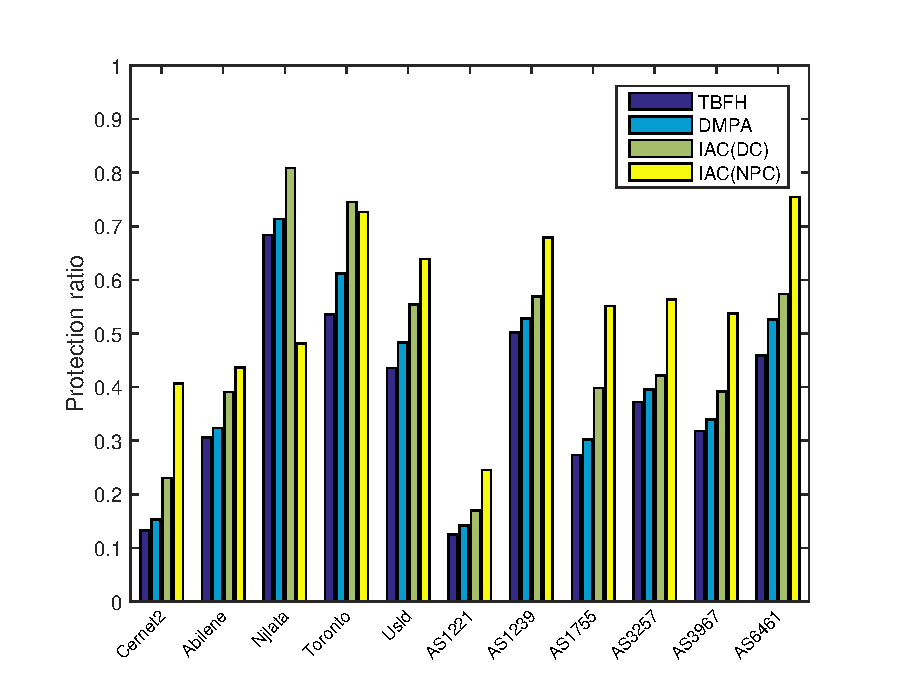
\includegraphics[width=\textwidth]{protectionratioreal}
                \caption{In real network topologies}
                \label{prreal}
        \end{subfigure}
        \caption{Comparison on the protection ratio in different topologies}
        \label{theoremexample}
\end{figure*}

\begin{figure*}[t!]
        \centering
        \begin{subfigure}[b]{0.32\textwidth}
                \centering
                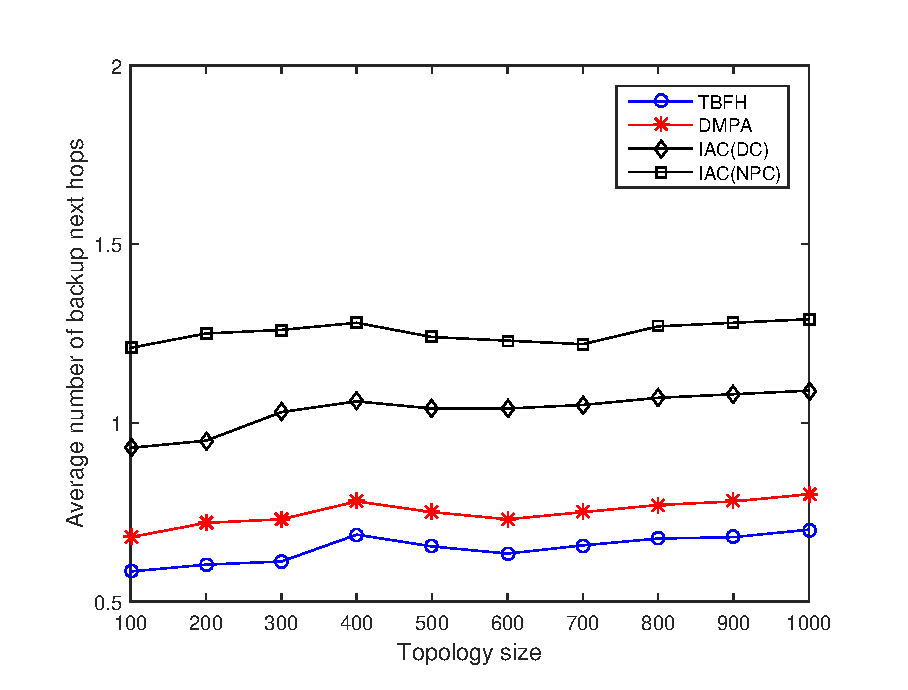
\includegraphics[width=\textwidth]{topnum}
                \caption{Varying topology size in Brite topologies}
              \label{topnumber}
        \end{subfigure}
        \begin{subfigure}[b]{0.32\textwidth}
                \centering
                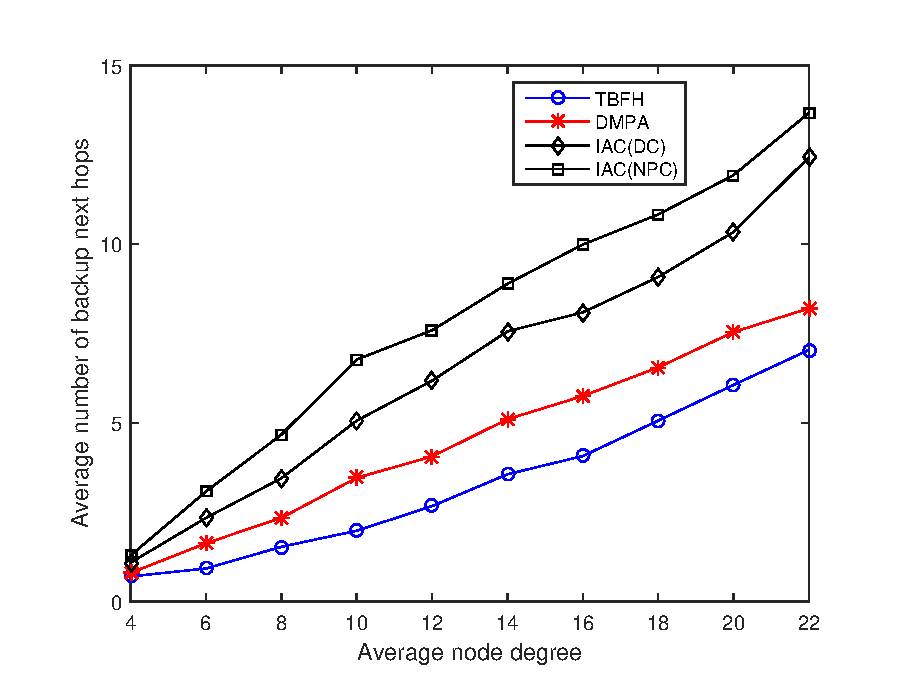
\includegraphics[width=\textwidth]{generatenum}
                \caption{Varying node degree in Brite topologies}
                \label{degnumber}
        \end{subfigure}
         \begin{subfigure}[b]{0.32\textwidth}
                \centering
                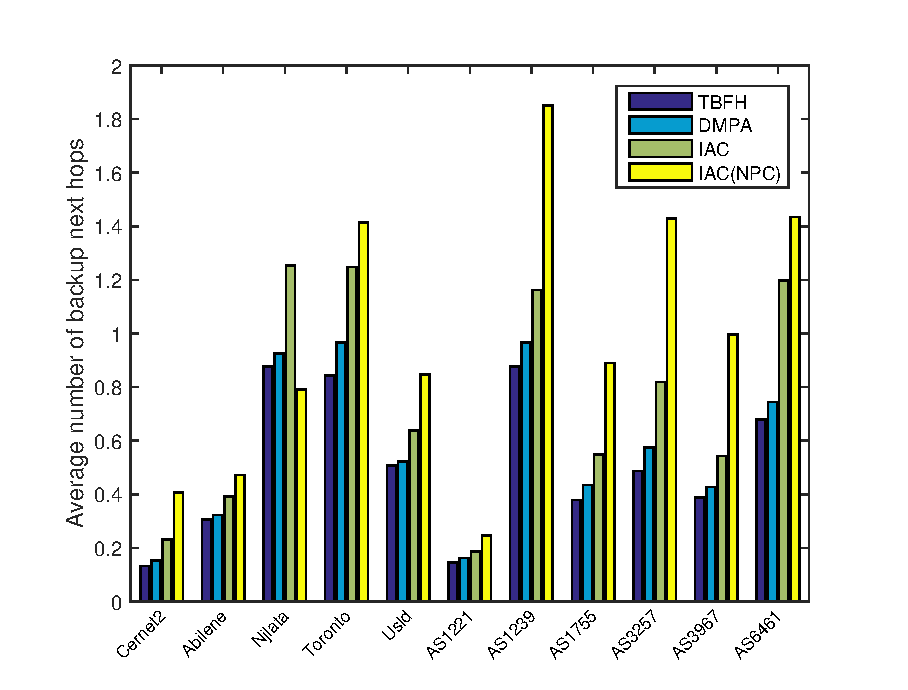
\includegraphics[width=\textwidth]{realnum}
                \caption{In real network topologies}
                \label{realnumber}
        \end{subfigure}
        \caption{Comparison on the average number of alternate next hops in different topologies}
        \label{theoremexample}
\end{figure*}
\begin{figure*}[t!]
        \centering
        \begin{subfigure}[b]{0.32\textwidth}
                \centering
                \includegraphics[width=\textwidth]{Cernet2cumulative}
                \caption{Cernet2}
              \label{cernet2cumulative}
        \end{subfigure}
                 \begin{subfigure}[b]{0.32\textwidth}
                \centering
                \includegraphics[width=\textwidth]{TORONTOcumulative}
                \caption{Toronto}
                \label{TORONTOcumulative}
        \end{subfigure}
         \begin{subfigure}[b]{0.32\textwidth}
                \centering
                \includegraphics[width=\textwidth]{1239cumulative}
                \caption{AS1239}
                \label{1239cumulative}
        \end{subfigure}
        \caption{Cumulative distribution of the
number of backup next hops on different topologies}
        \label{theoremexample}
\end{figure*}
\iffalse
\begin{figure}[t]
\centering
\includegraphics[width=3in]{degcomputationoverhead}
\caption{Computation overhead on generated topologies when topology size is 200}
\label{nodedegree6}
\end{figure}
\begin{figure}[t]
\centering
\includegraphics[width=3in]{realcomputationoverhead}
%\includegraphics[width=3in]{lfaexample}
\caption{Computation overhead on real and measured topologies}
\label{realtopologytime}
\end{figure}
\fi
\iffalse
Theoretical analysis has indicated that the time complexity of IAC is less than that of building of a shortest path tree, which has a great advantage over Naive, TBFH and DMPA.\fi
In order to verify the computational performance, we make simulations on different topologies. In this section, we evaluate the computational overhead of different algorithms. In order to avoid the uncertain factors impact the algorithm��s performance. The computational overhead of an algorithm is defined as the ratio of computation time of the algorithm to that of SPF (shortest path first).

\iffalse
\begin{figure}[t]
\centering
\includegraphics[width=3in]{rocketcomputationoverhead}
%\includegraphics[width=3in]{lfaexample}
\caption{Computation overhead on  measured topologies}
\label{rockettopologytime}
\end{figure}
\fi
Fig. \ref{topcom} shows relationship between the computation overhead and topology size on generated topologies when the average node degree is 6.
Fig. \ref{nodedegreecom} presents the relationship between the computation overhead and average node degree on generated topologies when the topology size is 500.
As the average node degree increases, the computation overhead of Naive increases accordingly. And also IAC has the highest performance among all the algorithms. Therefore, the above experiment results are consistent with the theoretical analysis described above.

Fig. \ref{realtopologytime} indicates the computational overhead obtained by different algorithms on real and Rocketfuel topologies. From the Fig. \ref{realtopologytime}, we can see that IAC has the lowest computation overhead among all the algorithms. The computation overhead of IAC is less than computing a SPT, while DMPA need to construct a SPT and TBFH need to compute two SPTs. The computation overhead of Naive is proportionally to the average node degree of the network.
\iffalse
\begin{figure}[t]
\centering
\includegraphics[width=3in]{tscomputationoverhead}
\caption{Computation overhead on generated topologies when average node degree is 6}
\label{topologysize200}
\end{figure}
\fi


\iffalse
\begin{figure*}[t]
        \centering
        \begin{subfigure}[b]{0.32\textwidth}
                \centering
                \includegraphics{abilenedeploy}
                \caption{$T_{c}$}
              \label{spttree}
        \end{subfigure}
        \begin{subfigure}[b]{0.32\textwidth}
                \centering
                \includegraphics{exodusdeploy}
                \caption{$T'_{c}$ when $L(c,a)=0$}
                \label{spttreechange1}
        \end{subfigure}
         \begin{subfigure}[b]{0.32\textwidth}
                \centering
                \includegraphics{sprintdeploy}
                \caption{$T'_{c}$ when $L(c,b)=0$}
                \label{spttreechange2}
        \end{subfigure}
        \caption{An example for explaining some Theorems}
        \label{theoremexample}
\end{figure*}
\fi
\iffalse
\begin{figure}[t]
\centering
\includegraphics[width=3in]{abilenedeploy}
\caption{Incremental Deployment on Abilene}
\label{abilene}
\end{figure}

\begin{figure}[t]
\centering
\includegraphics[width=3in]{exodusdeploy}
\caption{Incremental Deployment on Exodus}
\label{exodus}
\end{figure}

\begin{figure}[t]
\centering
\includegraphics[width=3in]{sprintdeploy}
\caption{Incremental Deployment on Sprint}
\label{sprint}
\end{figure}

\begin{figure}[t]
\centering
\includegraphics[width=3in]{top1000}
\caption{Incremental Deployment on Generated Topologies When Topology Size=1000}
\label{top100avi}
\end{figure}
\fi
\iffalse
\begin{figure}[t]
\centering
\includegraphics[width=3in]{topodeploy200}
\caption{Incremental Deployment on Topology=200}
\label{abilene}
\end{figure}

\begin{figure}[t]
\centering
\includegraphics[width=3in]{topodeploy500}
\caption{Incremental Deployment on Topology=500}
\label{exodus}
\end{figure}

\begin{figure}[t]
\centering
\includegraphics[width=3in]{topodeploy1000}
\caption{Incremental Deployment on Topology=1000}
\label{sprint}
\end{figure}
\fi
\iffalse
Fig. \ref{topologysize200} illustrates the relationship between the computation overhead and topology size on generated topologies when the average node degree is 6. As Fig. \ref{topologysize200} shows, the computation overhead of all the algorithms does not depend on the topology size. The computation overhead of IAC is lowest among all the algorithms.
\fi


\iffalse
 \begin{table}[h]
\centering
\renewcommand{\arraystretch}{1}
\caption{Computation time for Real Topologies}
\label{comparison}
\begin{tabular}{c|c|c|c|c|c|c}
\hline
&\multirow{2}{*}{Network}& \multicolumn{5}{|c}{Computation time ($\upmu$s)} \\
\cline{3-7}
& & OSPF &LFC & TBFH & MNP&MNP-e\\
\hline
Real& Abilene& 6.82&7.27 & 6.97 & 6.83&6.52\\
\hline
\multirow{3}{*}{Measured}& Exodus & 44.36 &128.29&88.76&50.23 &42.34\\
\cline{2-7}
& Telstra & 49.45 &163.43&100.34&54.34&46.23 \\
\cline{2-7}
& Tiscali & 79.45 &398.34&183.56&83.45 &75.34\\
\cline{2-7}
& Sprint &  140.23&906.78 &368.12 & 150.12 &137.34\\
\hline

\end{tabular}
\end{table}
\fi
\subsection{Protection ratio and the cumulative distribution of the
number of backup next hops}
In this section, we will use the protection ratio  and the average number of backup next hops to measure the path diversity of different algorithms.
The protection ratio is defined as
\begin{equation}
Pr=\frac{\sum\limits_{c,d\in V, c\neq d}{K(c,d)}}{|V|*(|V|-1)}
\end{equation}
\begin{equation}
K(c,d)=\begin{cases}
1&\mbox{$|N_c(d)|\geq 2$}\\
0&\mbox{$|N_c(d)|=1$}
\end{cases}
\end{equation}
The average number of backup next hops
describes the number of opportunities packets can be deflected off the
shortest path.
For both of the above two metrics, larger is better.

Fig. \ref{prtop} shows relationship between the computation overhead and topology size on generated topologies when the average node degree is 6.
Fig. \ref{prd} presents the relationship between the protection ratio and average node degree on generated topologies
when the topology size is 500.
Fig. \ref{prreal} depicts the protection ratio obtained by different algorithms on real and measured topologies.
Fig. \ref{topnumber} shows the average number of backup next hops obtained by different algorithms on generated topologies when the average node degree is 6.
Fig. \ref{degnumber} shows the average number of backup next hops obtained by different algorithms on generated topologies when the topology size is 500.
Fig. \ref{realnumber} depicts  the average number of backup next hops obtained by different algorithms on real and measured topologies.
Fig. \ref{cernet2cumulative}, \ref{TORONTOcumulative} and  Fig. \ref{1239cumulative} show
the cumulative distribution of the  number of backup next hops for CERNET2 , TORONTO and AS1239 topologies.
\iffalse
\begin{figure}[t]
\centering
\includegraphics[width=3in]{protectionratiodegree}
\caption{Protection ratio on generated topologies when topology size is 200}
\label{prd}
\end{figure}
\begin{figure}[t]
\centering
\includegraphics[width=3in]{protectionratioreal}
\caption{Protection ratio on real and measured topologies}
\label{prreal}
\end{figure}
\fi
\iffalse
\begin{figure}[t]
\centering
\includegraphics[width=3in]{protectionratiorocket}
\caption{Protection ratio on measured topologies}
\label{prrocket}
\end{figure}
\fi
\iffalse
\begin{figure}[t]
\centering
\includegraphics[width=3in]{generatenum}
\caption{Average number of backup next hops on real and measured topologies}
\label{generatenumber}
\end{figure}
\begin{figure}[t]
\centering
\includegraphics[width=3in]{realnum}
\caption{Average number of backup next hops on real and measured topologies}
\label{realnumber}
\end{figure}
\fi
\iffalse
\begin{figure}[t]
\centering
\includegraphics[width=3in]{rocketnum}
\caption{Average number of backup next hops on measured topologies}
\label{rocketnumber}
\end{figure}
\fi


\iffalse
\begin{figure}[t]
\centering
\includegraphics[width=3in]{TORONTOcumulative}
\caption{Cumulative  distribution of the number of backup next hops on Toronto topology}
\label{TORONTOcumulative}
\end{figure}
\begin{figure}[t]
\centering
\includegraphics[width=3in]{1239cumulative}
\caption{Cumulative  distribution of the  number of backup next hops on AS1239 topology}
\label{1239cumulative}
\end{figure}

\fi
\begin{figure}[t]
\centering
\includegraphics[width=3in]{topavi}
\caption{Network availability on generated topologies when average node degree=6}
\label{avtop}
\end{figure}
\begin{figure}[t]
\centering
\includegraphics[width=3in]{nodedegree}
\caption{Network availability on generated topologies when topology size=500}
\label{avdeg}
\end{figure}

We made several conclusions. First, IAC is more
flexible than TBFH and DMPA. It has more deflection choices in all
the experiment networks. Second, the
larger networks can provide more opportunities to detour.
\iffalse
Last,
For IAC/IAC-NA and DC, more than
40\% of routers have more than one next hop in all simulated topologies.
and this advantage is more pronounced in large topologies.
From Fig. \ref{prreal}, Fig. \ref{prrocket} and Fig. \ref{prd}, we can see that INC, INC-NA and DC have the similar protection ratio, which have better performance than both of DMPA and TBFH.
\fi
\subsection{Network availability}
Since both of the above two metrics cannot accurately describe end-to-end network availability. Therefore, we will use network availability \cite{Geng2017Algebra} to measure the end-to-end availability of different algorithms in the next section.
\iffalse
 We formally define the network availability $A(G)$ as follows (similar to that in \cite{ReliabilityAnalysis}),
and use it as a main metric to evaluate the protection capability of different schemes.

The end-to-end availability of a source-destination ($s$-$d$) pair is defined as the
probability that the packets can be correctly forwarded from $s$ to $d$.
Assume that there exist $n$ different forwarding paths from $s$ to $d$,
the $i$-th which is denoted by $p_{i}(s,d)$.
We also use $P_{i}(s,d)$ to represent the set of links on the $p_{i}(s,d)$.
Further, let the event that $p_{i}(s,d)$ works be denoted by $A_{i}(s,d)$,
whose probability can be expressed as:
\begin{equation}\label{ir}
P(A_{i})=\prod\limits_{\forall (m,n) \in P_{i}(s,d)}{r(m,n)}
\end{equation}


According to the Inclusion-Exclusion principle \cite{feller},
the end-to-end availability of a source-destination pair can be expressed as:

\begin{equation}\label{asd}
A(s,d)=\sum\limits_{k=1}^{n}{(-1)^{(k-1)}S_k}
\end{equation}
where $S_k$ denote the sum of the probabilities that a unique set of $k$ paths
from $s$ to $d$ are simultaneously working, which is further expressed as:

\begin{eqnarray}\label{sk}
S_{k}&=&\sum\limits_{i<j< \cdots <k}{P(A_{i} \cap A_{j}\cdots \cap A_{k})} \nonumber \\
&=&\sum\limits_{i<j< \cdots <k} \left(\prod\limits_{ (m,n) \in P_{i}(s,d) \cup P_{j}(s,d) \cup \dots \cup P_{k}(s,d)}{r(m,n)}\right) \nonumber
\end{eqnarray}


Then, the network availability can be computed as

\begin{equation}
A(G)=\frac{\sum\limits_{s,d \in V, s \neq d}{A(s,d)}}{|V|*(|V|-1|)}
\end{equation}
\fi
\begin{table}[t]
\centering
%\normalsize
\footnotesize
%\small
%\renewcommand{\arraystretch}{1}
\caption{Network availability for real and measured topologies}
\label{Availability}
\begin{tabular}{c|c|c|c|c|c}
\hline
&\multirow{2}{*}{Network}& \multicolumn{4}{|c}{Network Availability($\%$)} \\
\cline{3-6}
& &Naive & TBFH &  DMPA&IAC\\
\hline
\multirow{5}{*}{Real}
& Cernet2&99.93 &97.37& 98.54 & 99.93\\
\cline{2-6}
& Abilene&99.97 &97.34& 98.63& 99.97\\
\cline{2-6}
& Njlata&99.93 &96.87& 97.81& 99.93 \\
\cline{2-6}
& Toronto&99.87 &97.65& 98.74& 99.87 \\
\cline{2-6}
& Usld&99.94 &97.34& 98.57 & 99.94\\
\cline{2-6}
\hline
\multirow{5}{*}{Measured}
& AS1221 & 99.94 &97.77&98.89&99.94 \\
\cline{2-6}
& AS1239 &  99.96&96.67 &98.75&99.96 \\
\cline{2-6}
& AS1755 &  99.98&97.98&98.56&99.98 \\
\cline{2-6}
& AS3257 & 99.91&96.35&98.03&99.91 \\
\cline{2-6}
& AS3967 & 99.94 &97.89&98.79&99.94 \\
\cline{2-6}
& AS6461 & 99.96 &97.58&98.69&99.96 \\
\cline{2-6}

\hline
\end{tabular}
\end{table}
Fig. \ref{avtop} shows the  relationship between the network availability and the topology size.
Fig. \ref{avdeg} illustrates the relationship between the network availability and the average node degree.
As Fig. \ref{avdeg} shows, as the average node degree increase, the network availability increases too. Note that when the average node degree increases, all schemes provide better protection results, while IAC/IAC-NA and DC are always much better than DMPA and TBFH.

Table \ref{Availability} provides the network availability provided by each protection scheme, on the real and measured topologies. From the results, we can see that IAC has a clear advantage over TBFH and DMPA, and has the same performance as Naive.




\iffalse
\subsection{Incremental Deployment}
In this paper, we have proposed IAC/IAC-NA,
which is compatible with nowadays link-state routing
protocol, such as OSPF and IS-IS.
ISPs can deploy the algorithm in two ways, full deployment and incremental deployment.
However, full deployment is a burden for all ISPs.
Therefore, incremental deployment is employed in practice.
In this section, we will address the incremental deployment problem.
A node-by-node incremental deployment scheme is highly preferred.
The optimal deployment can be defined as:\\
\textbf{Optimal Deployment:}
Given a graph $G(V,E)$ and a positive integer $k$, our objective is to find a deployment $M$ where, $M \subset V$ and $|M|$=$k$ such that network availability is maximized.
\iffalse
\begin{algorithm}[h]
\caption{GreedyDeploy($G, m$)}
\label{deployment1}
\begin{algorithmic}[1]
\STATE $M\leftarrow \emptyset$
\WHILE {$|M|\leq k$}
\STATE $a\leftarrow max(B(a,M))$
\STATE $M\leftarrow M\cup \{a\}$
\ENDWHILE
\RETURN $S$
\end{algorithmic}
\end{algorithm}
\fi

We first define a benefit function for a node with respect to
the nodes which have been deployed.
Let $a$ be an arbitrary node in the network.
The benefit of node $a$ with respect to $M$, which is the nodes have been already deployed, is
denoted by $B(a,M)$, which can be expressed as:
\begin{equation}\label{benefit}
B(a,M)=A(G,M\cup \{a\})-A(G,M)
\end{equation}

It has been proved in \cite{zhang2013rpfp} that
finding the optimal deployment is NP-Complete.
Because the Optimal Deployment is NP-Complete problem.
With regard to the large $k$ and large topologies, a straight-forward
exhaustive search is computationally unacceptable.

\iffalse
A  simple greedy heuristic algorithm (GreedyDeploy)
 for selecting nodes to be deployed. The inputs of algorithm  is $k$.
The outputs of the algorithm  is the optimal deployment $M$.
The algorithm  goes through several iterations,
in each iteration, we will select a node which  has the maximum benefit to be deployed.
\fi

\iffalse
We propose an improved algorithm (SimulateDeploy) roughly modeled
after the Simulated Annealing probabilistic metaheuristic \cite{retvari2011optimizing}.
The main idea is that we first randomly select the deployed nodes set $M$.
Then finding the best $S'$
and accept it if either $S'$ can obtain lager network availability
than $S$ or  the temperature $T$ of the system is sufficiently large.
As the algorithm progresses we gradually
reduce $T$, thus the system will increasingly tend to get stuck
 in a local optimal solution.


We develop  Algorithm \ref{deployment} to solve the Optimal Deployment issue.
First, we randomly select a set of $M$, $M \subset V$ and $|M|$=$k$ , and set an initial system temperature (lines 1-2).
Let tuple $(c,c')$ be a pair of nodes such that  $c \in M$  and  $c' \notin M$,
we unconditionally accept this $c'$ either if it is
better than the previous one or if a random number generated temperature is less than $T$ (lines 4-5).
This can guarantee the algorithm escape from a local minimum.
\fi
\begin{algorithm}[h]
\caption{SimulateDeploy}
\label{deployment}
\begin{algorithmic}[1]
\STATE $T\leftarrow T_0 $
\STATE generate the initial set $M$ randomly
\REPEAT
%\STATE $\forall c \in M  and  c' \notin M$
\IF {$A(G,(M-c) \cup c')>A(G,M)\wedge T>random(T_0)$ }
\STATE $M\leftarrow (M-c) \cup c'$
\ELSE
\STATE $T\leftarrow T-1$
\ENDIF
\UNTIL{$T>T_{0}\land$ no such $(c,c')$ exists}
\RETURN $M$
\end{algorithmic}
\end{algorithm}

We propose an improved approximate algorithm roughly modeled
after the Simulated Annealing probabilistic metaheuristic \cite{retvari2011optimizing}.
The main idea is that we first select $M$, which is the solution generated randomly.
Then finding the best solutions
and accept it if either they can obtain lager network availability
than the former one or  the temperature $T$ of the system is sufficiently large.
As the algorithm progresses we gradually
reduce $T$, thus the system will increasingly tend to get stuck
in a good quality local minimum.
We develop  Algorithm \ref{deployment} to solve the Optimal Deployment issue.
The inputs of Algorithm \ref{deployment} is $k$.
The outputs of the Algorithm \ref{deployment} is the optimal deployment $M$.
First, we generate a set of $M$ for $M \subset V$ and $|M|$=$k$ randomly, and set an initial system temperature (lines 1-2).
Let tuple $(c,c')$ be a pair of nodes such that  $c \in M$  and  $c' \notin M$,
we unconditionally accept this $c'$ either if it is
better than the previous one or if a random number generated temperature is less than $T$ (lines 4-5).


Our proposed algorithm is compatible with the currently deployment intra-domain routing protocol.
In this section, we will show the relationship between the number of deployed nodes and network availability. In our experiment, we implement Algorithm \ref{deployment} respectively on real and generated topologies.
We repeated ten experiments, the final value for each topology is the average of the results.

Fig. \ref{abilene}, Fig. \ref{exodus}  and Fig. \ref{sprint} depict the relationship between the number of deployed nodes and network availability in  real networks and measured  topologies,
while Fig. \ref{top100avi} shows  the relationship between the number of deployed nodes and network availability in generated topology when the topology size is 1000.
Note that, as the node deployed ratios increases, the network availability increase too, our proposed algorithm can provide comparable performance to that of DC. Through this experiment, we will give ISPs a recommendation that they
can give priority to the deployment of some key nodes, and finally the whole network deployment.
In the actual deployment, we can give priority to the deployment of key nodes.
%We can also see that when a deployment on only 40\% nodes already increase the network availability clearly.
\fi


\section{Conclusion}\label{conclusion}
This paper is mainly focusing on the problem that how to efficiently
and effectively deploy LFA on ISPS' networks.
To this end, an incremental alternates computation with negative augmentation algorithm (IAC-NA) based on Incremental Shortest Path First
Algorithm was proposed.
Unlike majority of
schemes proposed in the literature, IAC-NA does not need to construct many SPTs on a node, which would entail significant computation overhead.
We also established the correctness of our scheme,
together with some other important properties. On top of that,
simulation results using several realistic network instances
gave evidence that IAC-NA  is very competitive in terms of
network availability as well.
The simulation results showed that IAC-NA can achieve
the same network availability as  the state-of-the-art LFA with small computation overhead.

In the future, we will focus on studying the link failure characteristics.
We believe that accurate link failure model will accurately improve  the performance evaluation.
We will use virtualization technology to deploy our algorithms on
CERNET2, which is the China Education and Research network.

%\section{Acknowledgement}\label{acknowledge}
This work is partially supported by the National Natural Science
Foundation of China (Grant No. 61702315).


\iffalse
\begin{biography}{genghaijun.eps}{Haijun Geng}  received the B.E, M.E. and Ph.D  degrees from Yantai University, Capital Normal University and Tsinghua University, in 2008, 2011 and 2015 respectively. He is now working in the School of Software Engineering, Shanxi University. His research
interests include future Internet architecture and largescale Internet routing.
\end{biography}
\epsfysize=3.2cm
\begin{biography}{shixingang.eps}{Xingang Shi} received the B.S. degree from
Tsinghua University and the Ph.D. degree from
the Chinese University of Hong Kong. He is now
working in the Institute for Network Sciences
and Cyberspace at Tsinghua University. His research interests include network measurement
and routing protocols.
\end{biography}
\epsfysize=3.2cm
\begin{biography}{wangzhiliang.eps}{Zhiliang Wang} received the B.E., M.E. and Ph.D.
degrees in computer science from Tsinghua University, China in 2001, 2003 and 2006 respectively. Currently he is an associate professor in the
Institute for Network Sciences and Cyberspace
at Tsinghua University. His research interests include formal methods and protocol testing, next
generation Internet, network measurement.
\end{biography}
\epsfysize=3.2cm
\begin{biography}{yinxia.eps}{Xia Yin} received the B.E., M.E. and Ph.D. degrees
in Computer Science from Tsinghua University
in 1995, 1997 and 2000 respectively. She is a
full professor in Department of Computer Science
and Technology at Tsinghua University. Her research interests include future Internet architecture, formal method, protocol testing and largescale Internet routing.
\end{biography}
\epsfysize=3.2cm
\begin{biography}{yinshaoping.eps}{Shaoping Yin}
received the B.E. degree in information engineering from Sichuan University in 1987 and M.E. degree in signal processing from Chinese Academy of Sciences in 1997 respectively.  He is an associate professor in School of Software Engineering, Shanxi University.
His research interests include routing protocols, network security and cloud computing.
\end{biography}
\fi
\bibliographystyle{IEEEtran}
\bibliography{multipath}
\end{document}

